\documentclass[pdflatex,sn-apa]{sn-jnl}
\geometry{text={160mm,240mm},top=25mm}
\usepackage{graphicx}%
\usepackage{multirow}%
\usepackage{amsmath,amssymb,amsfonts}%
\usepackage{amsthm}%
\usepackage{mathrsfs}%
\usepackage[title]{appendix}%
\usepackage{xcolor}%
\usepackage{textcomp}%
\usepackage{manyfoot}%
\usepackage{booktabs}%
\usepackage{array}%
\usepackage{algorithm}%
\usepackage{algorithmicx}%
\usepackage{algpseudocode}%
\usepackage{listings}%

\raggedbottom
\makeatletter\NAT@longnamesfalse\makeatother
\begin{document}

\title{Carbonatite-hosted REE prospectivity under extreme label scarcity in Canada: national-scale sampling and transferability, and a semi-supervised deviation network in three geological provinces}

\author*[1]{\fnm{Miaozhou} \sur{Tang}}\email{miaozhou.tang25@imperial.ac.uk}

\author[1]{\fnm{Junlin} \sur{Fang}}\email{junlin.fang22@imperial.ac.uk}

\author[1]{\fnm{Chetan} \sur{Nathwani}}\email{chetan.nathwani@imperial.ac.uk}

\affil*[1]{\orgdiv{Department of Earth Science and Engineering}, \orgname{Imperial College London}, \orgaddress{\street{South Kensington Campus}, \city{London}, \postcode{SW7 2AZ}, \country{United Kingdom}}}


\abstract{Carbonatites are the primary geological sources of rare earth elements (REEs), yet their prospectivity mapping is constrained by extreme label scarcity, the diverse geological settings hosting these deposits, the absence of reliable negative labels and limited model interpretability. Recent national-scale models report test AUCs above 0.9, but use augmented labels, negatives from the ground least similar to the occurrences and random splits. This study tests that design and the transferability of models between geological provinces, and then whether a semi-supervised anomaly-detection model, the Deviation Network (DevNet), offers advantages over Random Forest (RF), XGBoost and positive–unlabelled learners in the Superior Province, with the Cordilleran Orogen and Grenville Province as contrasts. Geophysical rasters and their derivatives, proximity-to-structure features and H3-grid geology were extracted per province. All models were trained on the occurrences together with an identical 5,000-point background sample, evaluated on a disjoint random-background set with pooled out-of-fold average precision (AP) and area under the ROC curve (AUC) under repeated random and 50–200 km spatially blocked cross-validation, and interpreted with SHapley Additive exPlanations (SHAP). Rebuilt on national data, the earlier design yields a test AUC of 1.000, which falls to 0.903 (AP 0.292) once labels are not augmented and negatives are drawn at random, and models do not transfer between provinces. In Superior, DevNet achieves the highest AP under both random (0.38) and spatially blocked (0.37–0.22) cross-validation, and the regional ordering (Superior > Cordillera > Grenville) agrees with previous studies. Carbonatite prospectivity models should therefore be built and validated within individual provinces, where semi-supervised methods match the reality that unexplored ground is not proven barren.}

\keywords{Mineral prospectivity mapping, Rare earth elements, Carbonatite, Deviation network, Random Forest, Positive--unlabelled learning, Spatial cross-validation}

\maketitle

%% ===================================================================
\section{Introduction}\label{sec:intro}

Rare earth elements (REEs) are critical to low-carbon energy, electronics and defence technologies, yet economic concentrations are geologically uncommon \citep{Wang2020}. Most REE resources are hosted by carbonatites and associated alkaline intrusions, whose distinctive but partly overlapping geophysical and geochemical signatures make them natural targets for data-driven mineral prospectivity mapping (MPM; \citealp{Verplanck2014,Simandl2018}). In Canada, however, confirmed carbonatite-hosted REE occurrences are few and spatially clustered (Fig.~\ref{fig:study}): after near-duplicates are merged, a single geological province holds between about ten and thirty of them.

Two properties of this problem undermine standard supervised classification. First, positives are extremely scarce: mineralisation is a rare event \citep{Xiong2018}, known occurrences are only a partial and biased sample of the mineral system \citep{Coolbaugh2007,Parsa2021,Zuo2021}, and under $k$-fold cross-validation each fold holds only a handful of them, so any estimate is dominated by which occurrences happen to be held out. Second, there are no true negatives. Ground without a recorded occurrence is unexplored rather than barren, and designating it negative is an arbitrary modelling choice whose outcome depends on which background points are drawn \citep{Zuo2020}. Together these properties motivate positive--unlabelled (PU) and semi-supervised anomaly-detection formulations, in which mineralised sites are treated as rare anomalies relative to a large, mostly barren but unlabelled population \citep{Chen2019,Xiong2016,Xiong2021,Bekker2020,Luo2026}.

The Deviation Network (DevNet; \citealp{Pang2019}) is a semi-supervised deep anomaly detector that learns an anomaly score from a few labelled anomalies and a large unlabelled pool, pulling the scores of unlabelled data towards a Gaussian reference while pushing labelled anomalies a fixed margin above it. \citet{Luo2026} adapted it to MPM (DEEP-SEAM), encoding geology as distances to mapped units and adding neighbourhood statistics of the evidence layers. Whether such a model outperforms discriminative baselines when positives number in the low tens has not been tested under evaluation designs that control for the specific ways in which small, clustered label sets inflate scores. The closest prior study, a national-scale model of Canadian carbonatite-hosted REE $\pm$ Nb deposits \citep{Parsa2024}, reported test AUCs of 0.91--0.96 with random forests and convolutional neural networks (CNNs), the highest for a CNN. Its labels were augmented by replacing each occupied S2 grid cell with its four child cells, its negatives were drawn from the ground least similar to the positives, and it was evaluated by stratified random 70/30 splits of the augmented labels. A follow-up study recommended synthetic labels generated by generative adversarial networks (GANs) for the same commodity \citep{Parsa2025}. Each of these design choices can make the held-out test easier than prospecting new ground. A national model also answers a different question from a provincial one. Pooling every occurrence of a country raises the label count, but it mixes occurrences from geological provinces whose geophysical settings, and whose barren ground, differ completely; whether a model trained on such a pool predicts within any one province, and whether one province's occurrences say anything about another's, is rarely tested \citep{Ploton2020,Meyer2021}.

This study starts at the national scale. We rebuild the S2-grid design of \citet{Parsa2024} on national data, compare it with a design that keeps one label per occurrence, draws background at random and evaluates at a realistic prevalence, and test whether models transfer between geological provinces. Because they do not, the main part of the study models provinces separately: the Superior Province of the Canadian Shield, the province in which labels are scarcest relative to area, with the Cordilleran Orogen and Grenville Province modelled with the identical pipeline as contrasting cases. All analyses share one occurrence table and one input rule; inputs whose value depends on the extent of the study area are computed per geological province, so that a point has the same value nationally and provincially. We ask: (i) how much of the high AUC of the national S2-grid design comes from its sampling and augmentation, and do models transfer between provinces? (ii) within Superior, does DevNet outperform tree-based learners (RF and XGBoost) and positive--unlabelled learners once every model sees the same data and folds, and does any advantage survive spatially blocked validation? (iii) how much of the skill comes from geological map classes that mark known complexes? and (iv) can synthetic positives compensate for label scarcity? We close by interpreting the provincial models with SHapley Additive exPlanations (SHAP), using a rank-based rule for the direction of each feature's effect, and by checking the Superior maps against an untrained REE resource and the mapped Kapuskasing Structural Zone.

%% ===================================================================
\section{Geological setting and data}\label{sec:data}

\subsection{Carbonatite-hosted REE systems and their geophysical expression}\label{sec:mineral-system}

Carbonatites occur predominantly in Precambrian cratonic areas, and individual provinces record repeated emplacement over hundreds of millions of years, implying long-lived, episodically reactivated trans-lithospheric pathways \citep{Woolley2012}. A component of their REE endowment is attributed to subcontinental lithospheric mantle refertilised by REE- and CO$_2$-rich metasomatic fluids \citep{Hou2023,Yaxley2021}. Each element of this source--transport--trap system has a mappable geophysical proxy (Fig.~\ref{fig:mineral-system}). Depth to the lithosphere--asthenosphere boundary (LAB) indexes the thickness and edge geometry of the cratonic root that hosts the fertile mantle source, which exerts first-order control on magmatic ore systems \citep{Griffin2013,Groves2021,Hoggard2020}; Moho depth indexes crustal thickness; and proximity to faults and to the loci of maximum horizontal gravity and magnetic gradient (``worms''; \citealp{Hornby1999}) proxies the structures that channel ascending melts. At the emplacement site, dense and magnetic alkaline--carbonatite complexes produce positive gravity anomalies and intense circular to annular magnetic anomalies \citep{Thomas2016,Drenth2014}. Grey-level co-occurrence matrix (GLCM) textures summarise the local two-dimensional heterogeneity produced by such concentric patterns without assuming a target diameter \citep{Cooper2005,HallBeyer2017}, unlike explicit radial-symmetry detectors tuned to ring-complex size \citep{Aranha2021}.

\begin{figure}[t]
\centering
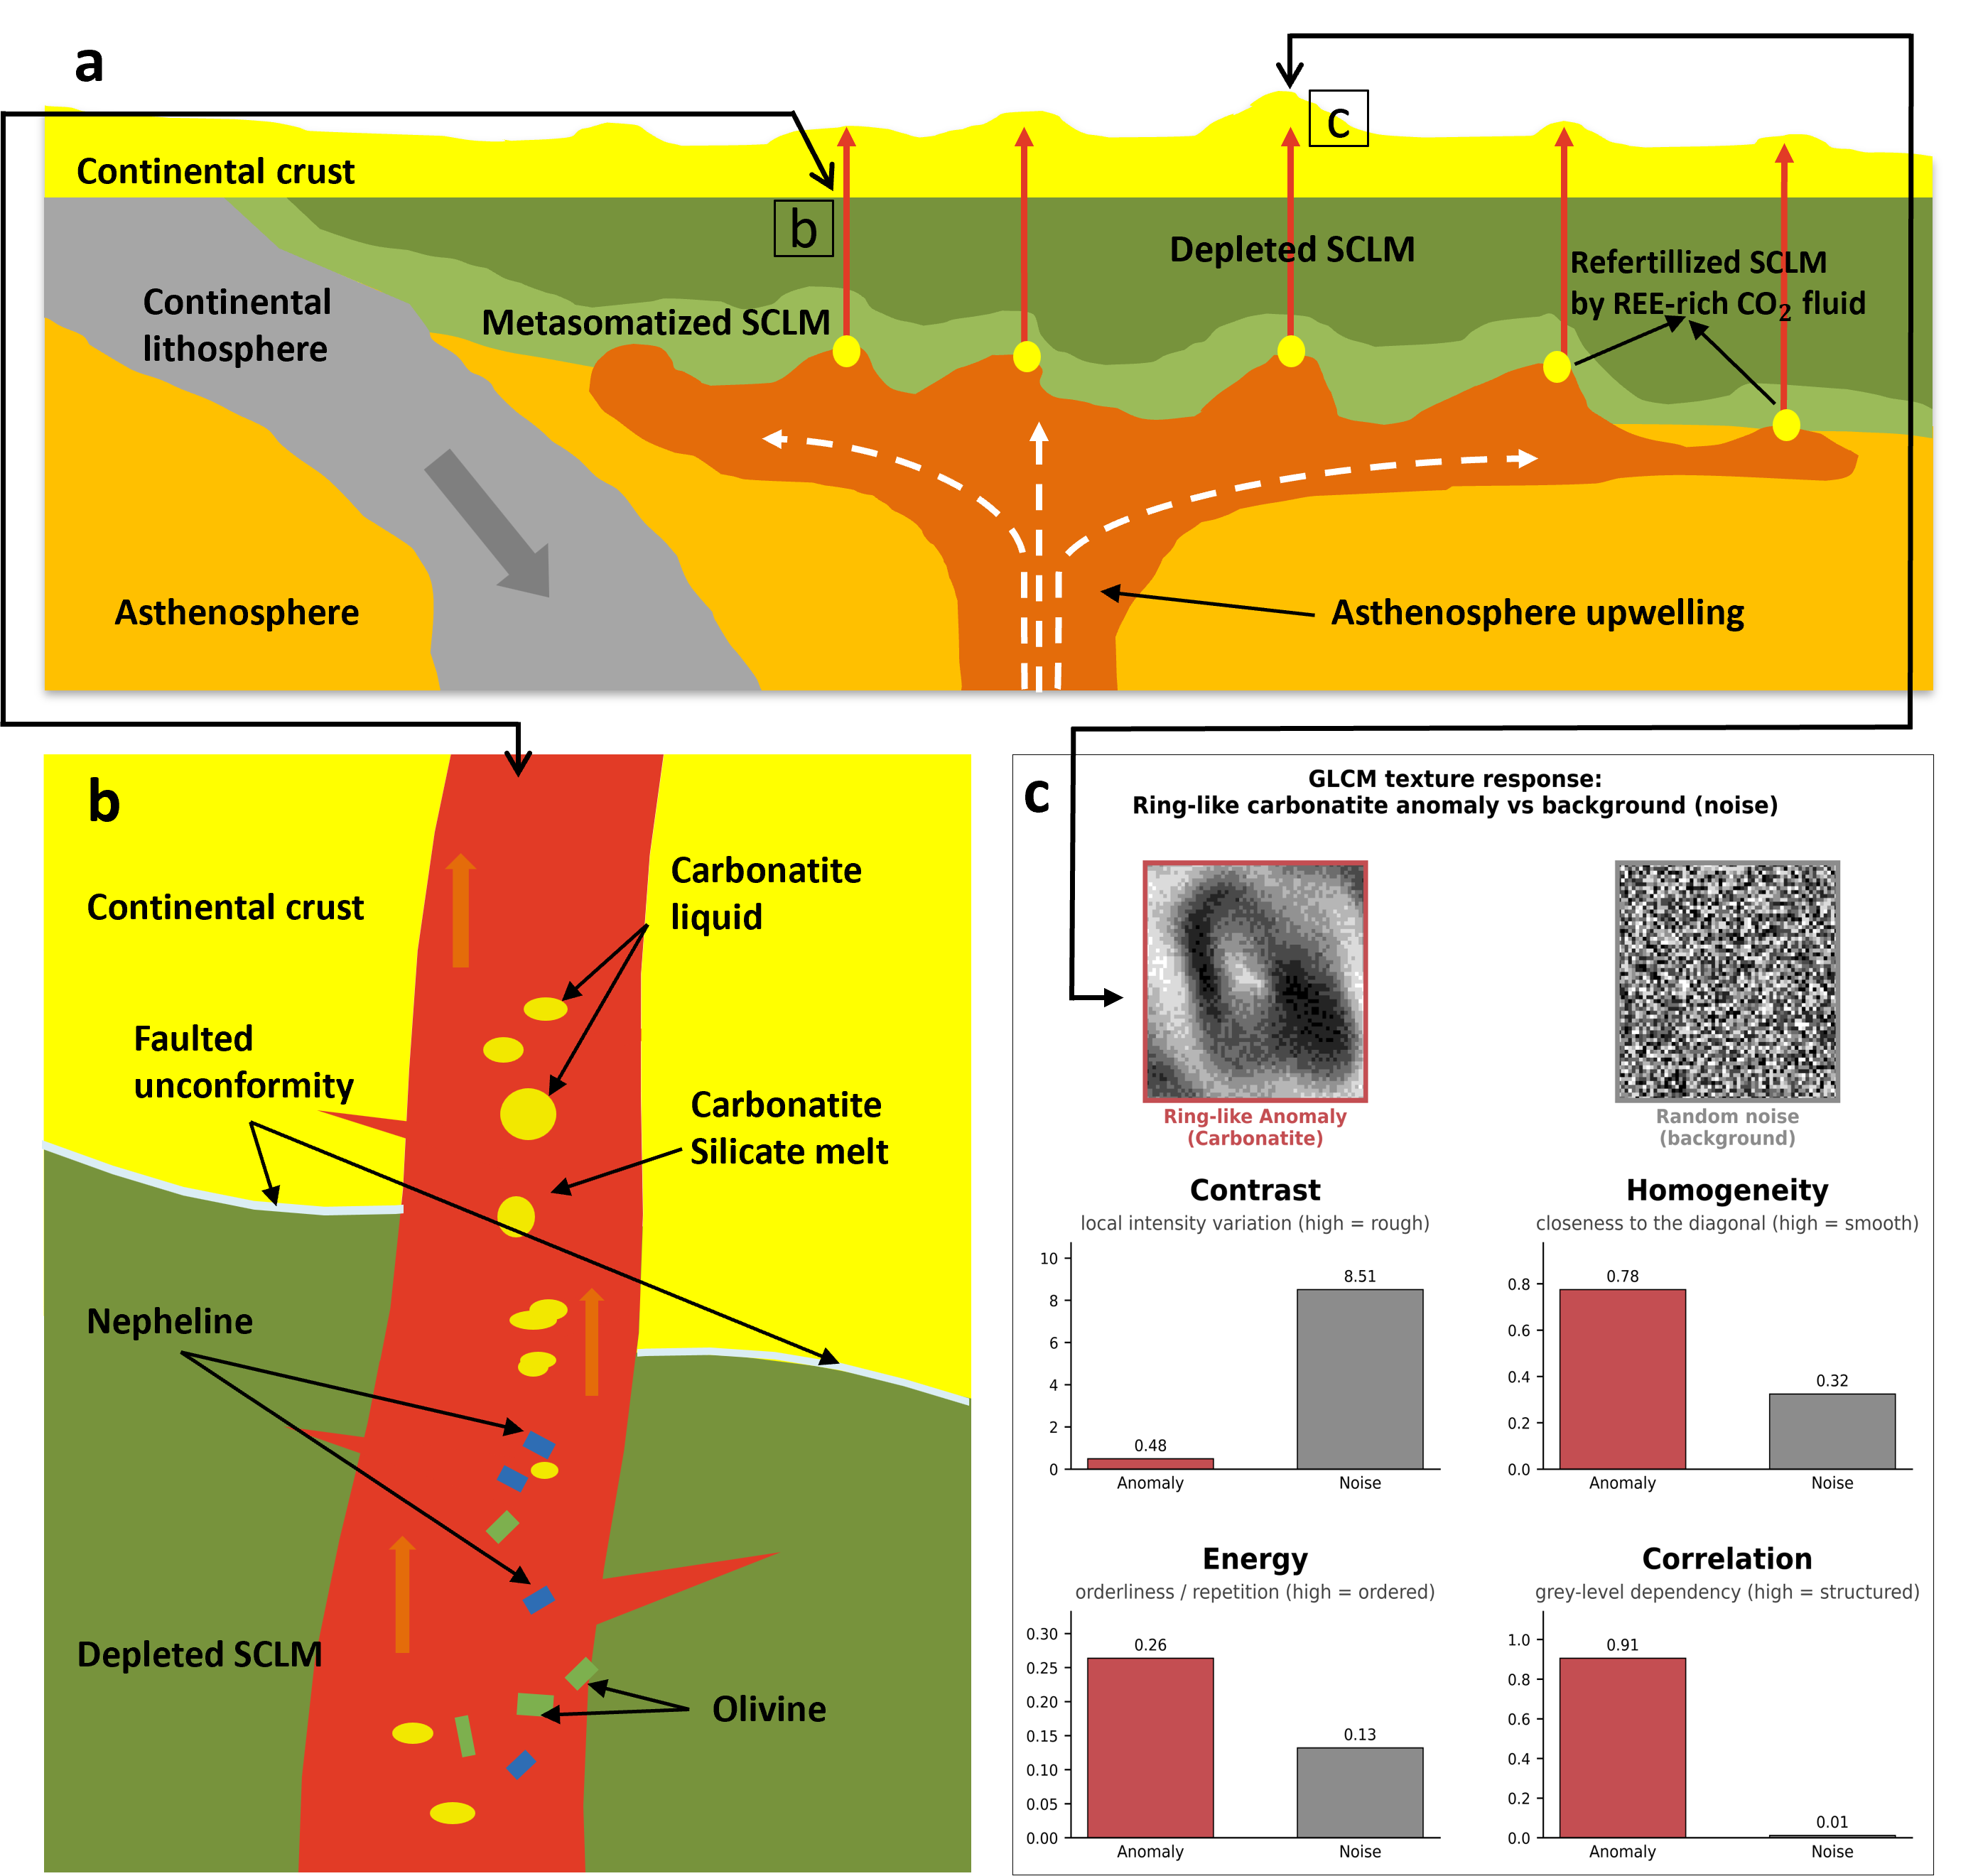
\includegraphics[width=0.85\textwidth]{figures/fig_mineral_system.png}
\caption{Source--transport--trap model for carbonatite-hosted REE systems and its geophysical proxies. (a) Source: refertilised subcontinental lithospheric mantle near the LAB at the craton margin, indexed by LAB depth and margin proximity; panel modified after \citet{Hou2023}. (b) Transport along trans-lithospheric faults, indexed by fault and worm proximity and Moho depth; modified after \citet{Yaxley2021}. (c) Trap: GLCM texture response of a ring-like anomaly and of random noise.}\label{fig:mineral-system}
\end{figure}

\subsection{Study areas}\label{sec:areas}

The national study area is the union of the onshore geological provinces, orogens and platforms of the Geological Map of Canada \citep[Map 1860A;][]{Wheeler1996}, without the continental shelves and oceanic crust (12.3 million km$^2$). The three provincial study areas are the Superior Province, the Grenville Province and the Cordilleran Orogen polygons of the same map. Carbonatite-hosted occurrences of the Phanerozoic, accreted Cordillera are geophysically distinct from those of the Canadian Shield \citep{Parsa2024}, which suggests that a single cross-terrane model would not transfer; Section~\ref{sec:res-national} tests this directly. Windows of one province enclosed by another and smaller than 2,000~km$^2$, such as the Churchill-basement windows of the Monashee and Malton complexes in the Cordillera, were assigned to the surrounding province.

The Superior Province is the world's largest Archean craton. Carbonatite--alkaline magmatism in the Canadian Shield clusters into episodes at about 2.68~Ga, 1.90--1.88~Ga and 1.16--1.08~Ga \citep{Rukhlov2010}, and in the Superior Province many of the complexes are aligned along crustal-scale structures, most prominently the Kapuskasing Structural Zone \citep[KSZ;][]{Percival1994,Gittins1967}. The 15 Superior occurrences used here (Fig.~\ref{fig:study}b) comprise a cluster around the Montviel and Lac Shortt carbonatites in the eastern Abitibi region of Qu\'ebec (Deposit/Prospect and Showing class) and occurrences dispersed across the southern and western Superior Province, including Nemegosenda Lake, Lackner Lake, Kapuskasing, Martison Lake, Prairie Lake and Carb Lake. The Superior Province thus combines the fewest occurrences per unit area of the three provinces with a spatial structure, one tight cluster plus scattered singletons, in which a model can either learn the cluster or learn what the scattered occurrences have in common.


\begin{figure}[t]
\centering
\includegraphics[width=0.55\textwidth]{overleaf_revised6/figures/REE distribution.png}\hfill
\vspace{0.3cm}
\includegraphics[width=0.42\textwidth]{overleaf_revised6/figures/occurrences-cordillera.jpg}\hfill
\vspace{0.3cm}
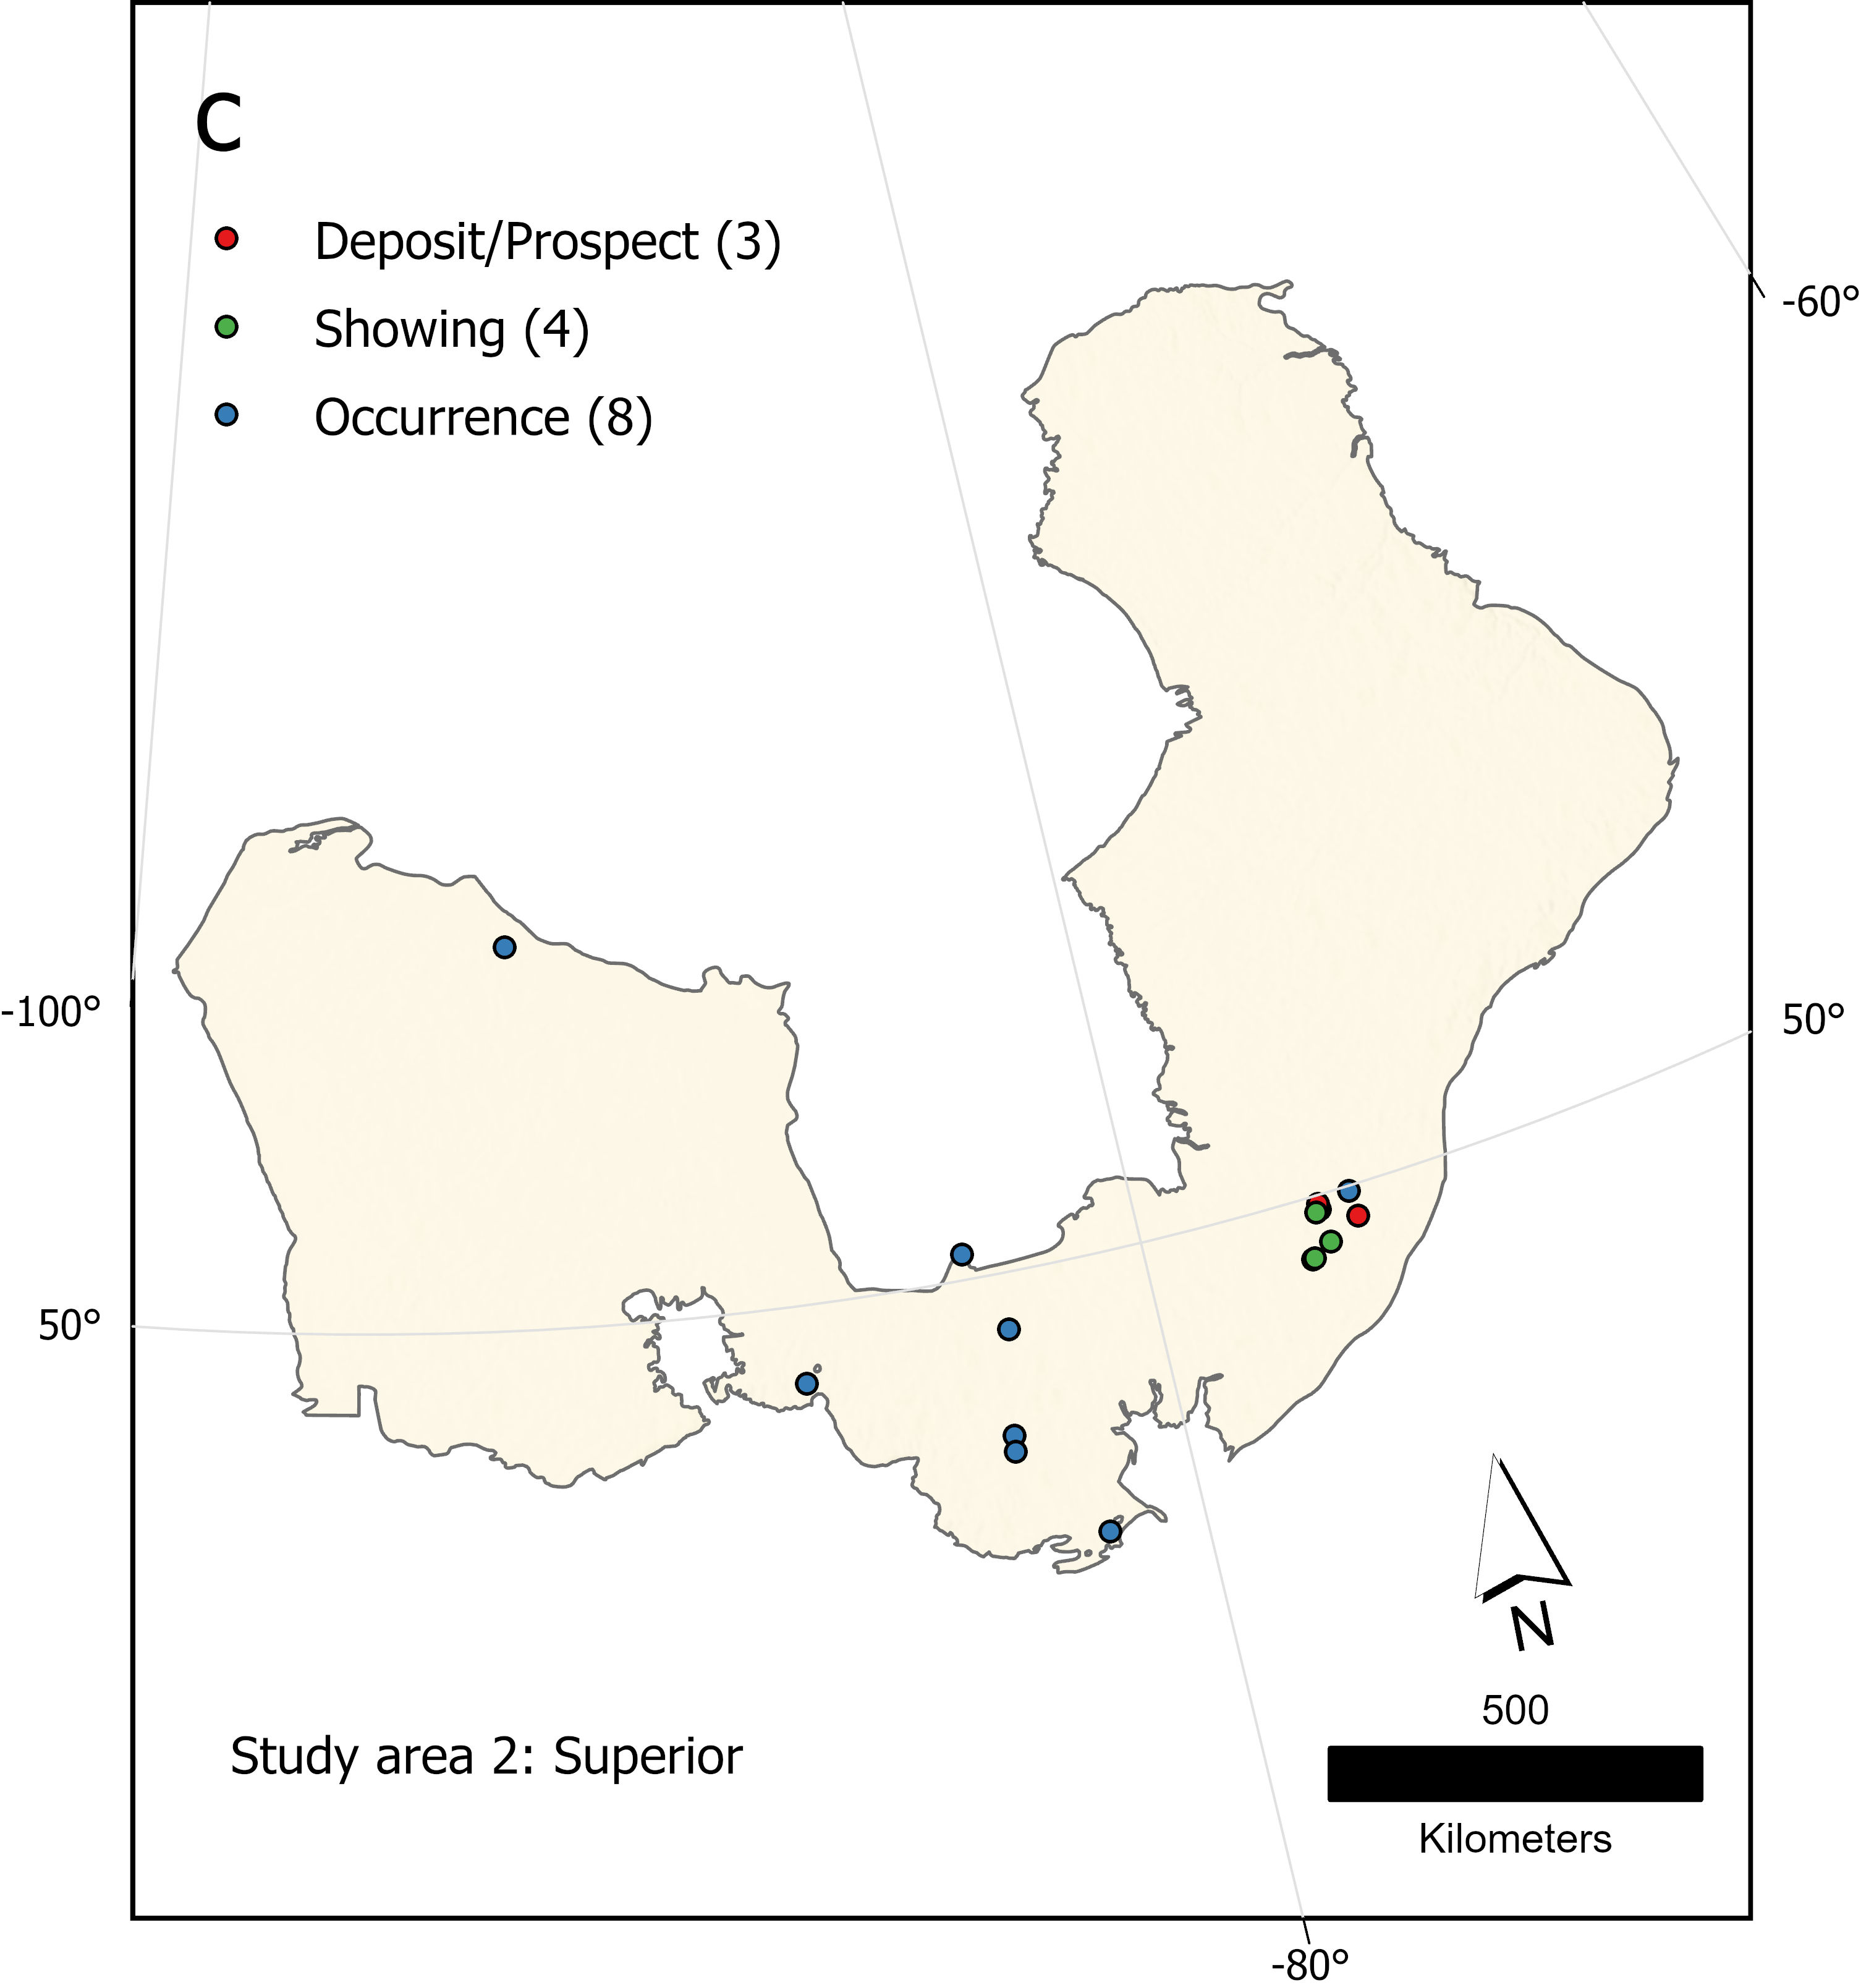
\includegraphics[width=0.427\textwidth]{figures/fig_study_superior.jpg}\hfill
\vspace{0.3cm}
\includegraphics[width=0.42\textwidth]{overleaf_revised6/figures/occurrences-grenville.jpg}
\caption{Comparison between the entire territory of Canada (a) and three priority areas (b-d) and known REE occurrences, illustrating the highly uneven and geologically constrained spatial distribution of REE mineralization across Canada. The coloured areas denote the regions covered by available data (the sampleable domain), within which sampling and prediction were confined. Occurrences compiled from two sources: \citet{Parsa2024} and \citet{Orris2018} Symbols denote the development status of each occurrence following \citet{Parsa2024}: Deposit/Prospect (promising to well-defined mineralisation with confirmed or potentially economic resources, requiring further detailed exploration to delineate), Showing (a higher likelihood of economic interest but requiring more exploration), and Occurrence (the most basic indication of minerals, often without economic viability). Only occurrences retained after deduplication and domain filtering were used as positive samples.}\label{fig:study}
\end{figure}

\subsection{Occurrence labels}\label{sec:labels}

Positive labels were compiled from the carbonatite-hosted records of the USGS global REE occurrence database \citep{Orris2018} and the occurrence table of \citet{Parsa2024}, totally 102 records across Canada. Alkaline-hosted occurrences were excluded after a preliminary leave-block-out classification showed them to be geophysically separable from carbonatite-hosted ones. Records within 2~km of each other were merged by single linkage, so that drill holes or zones of one deposit, listed once or in both sources, count once; without this step near-identical points from one deposit fall into both training and validation folds. Each occurrence keeps the development class of \citet{Parsa2024}: Deposit/Prospect, Showing or Occurrence. After merging and the data-coverage filter (Section~\ref{sec:domain}), the national label table holds 66 occurrences (Fig.~\ref{fig:study}a). Within the three study provinces, the same steps reduced 21, 13 and 51 pooled records to 15 (Superior), 12 (Grenville) and 27 (Cordillera) positives; the remaining 12 occurrences lie elsewhere in Canada.

\subsection{Geophysical and structural evidence layers}\label{sec:layers}

Table~\ref{tab:layers} lists the evidence layers. Seventeen national rasters cover the trap and the deep-architecture components: Bouguer gravity and its derivatives and filtered versions, total magnetic intensity and its differential reduction to the pole with derivatives \citep{Jobin2017,Miles2016}, together with long-wavelength gravity and magnetics, LAB and Moho depth from the Tri-National Critical Minerals Mapping Initiative release \citep{McCafferty2023}. The Bouguer anomaly (density 2.67~g\,cm$^{-3}$, terrain-corrected), its first vertical and total horizontal derivatives and the total magnetic intensity are the public Natural Resources Canada compilations \citep{Jobin2017,Miles2016}, regridded to 2~km (EPSG:3978) and 0.01$^\circ$. The other seven gravity and magnetic grids were computed from them for this study. The 40 and 100~km high-pass versions of the Bouguer anomaly apply a sixth-order Butterworth filter, $H(k) = [1 + (k_0/k)^6]^{-1}$ with $k_0$ the inverse of the cut-off wavelength, in the wavenumber domain. The magnetic field was reduced to the pole differentially \citep{ArkaniHamed1988,CooperCowan2005}: the total magnetic intensity was processed in 8$^\circ$ tiles with 4$^\circ$ overlap, each projected to a 1~km azimuthal equidistant grid, the reduction to the pole for induced magnetisation \citep{Blakely1995} was computed for nine combinations of inclination and declination spanning the tile and interpolated to the field direction at each node, taken from the International Geomagnetic Reference Field \citep[IGRF-13, epoch 2020.0;][]{Alken2021}, and the tiles were blended with cosine tapers. First vertical derivatives were computed in the wavenumber domain, total horizontal derivatives (THD) by central differences on metric cell sizes, and the tilt angle of a grid as the arctangent of its vertical over its total horizontal derivative \citep{Miller1994,Verduzco2004}; the THD tilt layers are the tilt angle of the THD grids. Two line layers (ancient passive margins, \citealp{BradleyDC2008}; faults) and four point layers (shallow and deep gravity and magnetic worms; \citealp{McCafferty2023}) enter as normalised proximities. GLCM contrast, homogeneity, energy and correlation were computed in 9$\times$9-pixel windows on all eleven gravity and magnetic grids; feature pruning (Section~\ref{sec:pruning}) removes the redundant ones. Following \citet{Luo2026}, the mean and standard deviation of the Bouguer anomaly, its 40~km high-pass, the reduced-to-pole magnetics and the total magnetic intensity within 10~km of each point were added as neighbourhood statistics. Radiometric grids (K, eU, eTh) were considered but not used, because their coverage of the study areas is incomplete and uneven; whole-rock geochemistry is too sparse to give a value at every map cell. The province polygons of \citet{Wheeler1996} define the study areas only; no distance-to-province-boundary feature was used.

\begin{sidewaystable}
\caption{Evidence layers by mineral-system component and mappable criterion, with their geometry, native resolution and source. Rasters were sampled at points in their native projection and resolution; line and point layers enter as normalised proximities.}\label{tab:layers}
\footnotesize
\setlength{\tabcolsep}{3pt}
\begin{tabular*}{\textwidth}{@{\extracolsep\fill}>{\raggedright\arraybackslash}p{1.7cm}>{\raggedright\arraybackslash}p{2.6cm}>{\raggedright\arraybackslash}p{3.5cm}>{\raggedright\arraybackslash}p{1.4cm}>{\raggedright\arraybackslash}p{2.4cm}>{\raggedright\arraybackslash}p{7.3cm}>{\raggedright\arraybackslash}p{2.9cm}}
\toprule
Component & Mappable criterion & Layer & Geometry & Native resolution & Description & Source \\
\midrule
Source & Mantle melting at craton margins & Ancient passive margins & Line & -- & Proximity to ancient passive margins & \citet{BradleyDC2008} \\
 & Lithospheric architecture & LAB depth & Raster & 0.1$^\circ$ ($\approx$11.1~km) & Depth to the lithosphere--asthenosphere boundary & \citet{McCafferty2023} \\
 & Deep crustal architecture & BA upward-continued 30~km & Raster & 0.031$^\circ$ ($\approx$3.4~km) & Bouguer gravity upward-continued by 30~km & \citet{McCafferty2023} \\
 & & BA upward-continued 30~km HGM & Raster & 0.031$^\circ$ ($\approx$3.4~km) & Horizontal-gradient magnitude of the upward-continued gravity & \citet{McCafferty2023} \\
 & & Deep-source RTP & Raster & 0.018$^\circ$ ($\approx$2.0~km) & Long-wavelength (deep-source) reduced-to-pole magnetics & \citet{McCafferty2023} \\
 & & Deep-source RTP HGM & Raster & 0.019$^\circ$ ($\approx$2.1~km) & Horizontal-gradient magnitude of the deep-source RTP & \citet{McCafferty2023} \\
\midrule
%% TODO(author): confirm the provenance of the fault compilation (KNOWN_ISSUES.md #3)
Transport & Crustal architecture & Moho depth & Raster & 0.25$^\circ$ ($\approx$27.8~km) & Depth to the Moho & \citet{McCafferty2023} \\
 & & Faults & Line & -- & Proximity to faults & \citet{McCafferty2023} \\
 & & Shallow gravity worms & Point & -- & Proximity to horizontal-gradient maxima of the Bouguer gravity & \citet{McCafferty2023} \\
 & & Deep gravity worms & Point & -- & Proximity to horizontal-gradient maxima of the 30~km upward-continued gravity & \citet{McCafferty2023} \\
 & & Shallow magnetic worms & Point & -- & Proximity to horizontal-gradient maxima of shallow magnetic sources & \citet{McCafferty2023} \\
 & & Deep magnetic worms & Point & -- & Proximity to horizontal-gradient maxima of deep magnetic sources & \citet{McCafferty2023} \\
\midrule
Trap & Gravity anomaly & Bouguer anomaly (BA) & Raster & 2~km & Bouguer anomaly (2.67~g\,cm$^{-3}$, terrain-corrected) & \citet{Jobin2017} \\
 & & BA 1VD & Raster & 2~km & First vertical derivative of the BA & \citet{Jobin2017} \\
 & & BA THD & Raster & 2~km & Total horizontal derivative of the BA & \citet{Jobin2017} \\
 & & BA THD tilt & Raster & 2~km & Tilt angle of the BA THD & This study \\
 & & BA high-pass 40~km & Raster & 2~km & 40~km high-pass (sixth-order Butterworth) of the BA & This study \\
 & & BA high-pass 100~km & Raster & 2~km & 100~km high-pass (sixth-order Butterworth) of the BA & This study \\
\cmidrule(l){2-7}
 & Magnetic anomaly & Total magnetic intensity (TMI) & Raster & 0.01$^\circ$ ($\approx$1.1~km) & Total magnetic intensity & \citet{Miles2016} \\
 & & DRTP & Raster & 0.01$^\circ$ ($\approx$1.1~km) & Differential reduction to the pole of the TMI & This study \\
 & & DRTP 1VD & Raster & 0.01$^\circ$ ($\approx$1.1~km) & First vertical derivative of the DRTP & This study \\
 & & DRTP THD & Raster & 0.01$^\circ$ ($\approx$1.1~km) & Total horizontal derivative of the DRTP & This study \\
 & & DRTP THD tilt & Raster & 0.01$^\circ$ ($\approx$1.1~km) & Tilt angle of the DRTP THD & This study \\
\cmidrule(l){2-7}
 & Anomaly geometry & GLCM textures & Derived & 9$\times$9-pixel window & Contrast, homogeneity, energy and correlation of each of the eleven gravity and magnetic grids & This study \\
 & & Neighbourhood statistics & Derived & 10~km radius & Mean and standard deviation of the BA, BA high-pass 40~km, DRTP and TMI & This study, after \citet{Luo2026} \\
\cmidrule(l){2-7}
 & Host architecture & Lithology, era, contacts & H3 grid & Resolution 7 ($\approx$4.9~km$^2$ cells) & Major lithology class and era of the cell (one-hot); flags for lithological and age contacts in the cell & \citet{Wheeler1996} \\
 & & Distances to generalised geology & Derived & -- & Distances to lithological and age contacts and to greenstone, mafic--ultramafic, high-grade metamorphic and sedimentary units (Section~\ref{sec:featuresets}) & This study, from \citet{Wheeler1996} \\
\botrule
\end{tabular*}
\end{sidewaystable}

\subsection{Geology}\label{sec:featuresets}

Geology enters from a hexagonal H3 grid (resolution 7, cells of about 5~km$^2$) attributed from the Geological Map of Canada \citep{Wheeler1996}. Each cell carries a major lithology class (for example Igneous Intrusive Alkalic or Metamorphic Gneiss Paragneiss), its dominant era, and flags for cells crossed by a lithological or an age (period) contact; each point takes the attributes of the cell that contains it. The lithology class enters as one-hot columns (a class gets its own column if at least 10 of the region's 5,000 training-background points fall in it; rarer classes share one), together with the era one-hot and the two contact flags. Following \citet{Luo2026}, geology also enters as distances (km) to six elements of a generalised map, from which every lithological unit smaller than 20 connected cells (about 100~km$^2$) and the alkalic-intrusion class were removed: lithological contacts, age contacts, greenstone (extrusive) units, mafic--ultramafic intrusions, high-grade metamorphic units and sedimentary units. After pruning (Section~\ref{sec:pruning}) the inputs number 57 in Superior (33 geophysical and structural layers, 14 of them GLCM textures, 3 neighbourhood statistics, 2 regional distances, 15 lithology columns, 2 era columns and 2 contact flags), 61 in Cordillera and 66 in Grenville.

At the scale of a carbonatite complex a bedrock map can mark the target itself: in Superior, 6 of the 15 occurrences fall on cells mapped as alkalic intrusive rock, against 16 of the 3,000 evaluation-background points (0.5\%). A mapped alkaline complex is legitimate evidence for an explorer, but a model can score well simply by looking it up. We therefore also report the models without the point-level map classes (the lithology, era and contact columns), keeping the geophysical and structural layers, neighbourhood statistics and regional distances (38, 37 and 41 inputs after pruning). This measures what the models achieve on ground where the map does not show a complex.

\subsection{Sampleable domain and background}\label{sec:domain}

Rasters were clipped to each study-area outline buffered outward by one GLCM window radius (8~km), so that windows near the boundary read real data, and sampling and prediction were restricted to the domain where every layer holds data and every texture window is computable. This domain covers 98.6\% of the Superior, 97.2\% of the Grenville and 73.5\% of the Cordilleran outline and 8.09 million km$^2$ (65.6\%) of Canada; one Cordilleran occurrence (Lempriere) and one St.~Lawrence Platform occurrence (Francon Quarry) fall outside it and were dropped. Background candidates are the nodes of a 0.1$^\circ$ grid inside the domain and more than 10~km from any known occurrence (19,371 in Superior). From these, two disjoint pools were drawn once per region at random: an evaluation background of 3,000 points and a training background of 5,000 points. Every model in this study is trained on the positives of its training fold plus the same 5,000 training-background points and scored on the held-out positives plus the same evaluation background. The prevalence in the scored pool is therefore 15/3,015 $\approx$ 0.5\% in Superior, which is the AP of a random ranking.

For the national analyses the same rules were applied to Canada as a whole. Inside the study provinces the national background points are provincial ones (in Cordillera and Grenville random subsets of them, so that the density matches Superior's), and elsewhere background was drawn at Superior's density, 41\% of the candidate nodes, with evaluation and training background split 3:5 as in each province. The national table holds 66 occurrences, 20,855 evaluation-background and 34,761 training-background points (prevalence 0.32\%).

%% ===================================================================
\section{Methods}\label{sec:methods}

Figure~\ref{fig:workflow} summarises the workflow. Code for every analysis, including the exact numbers in every table, is available in the repository listed under Code availability.

\begin{figure}[t]
\centering
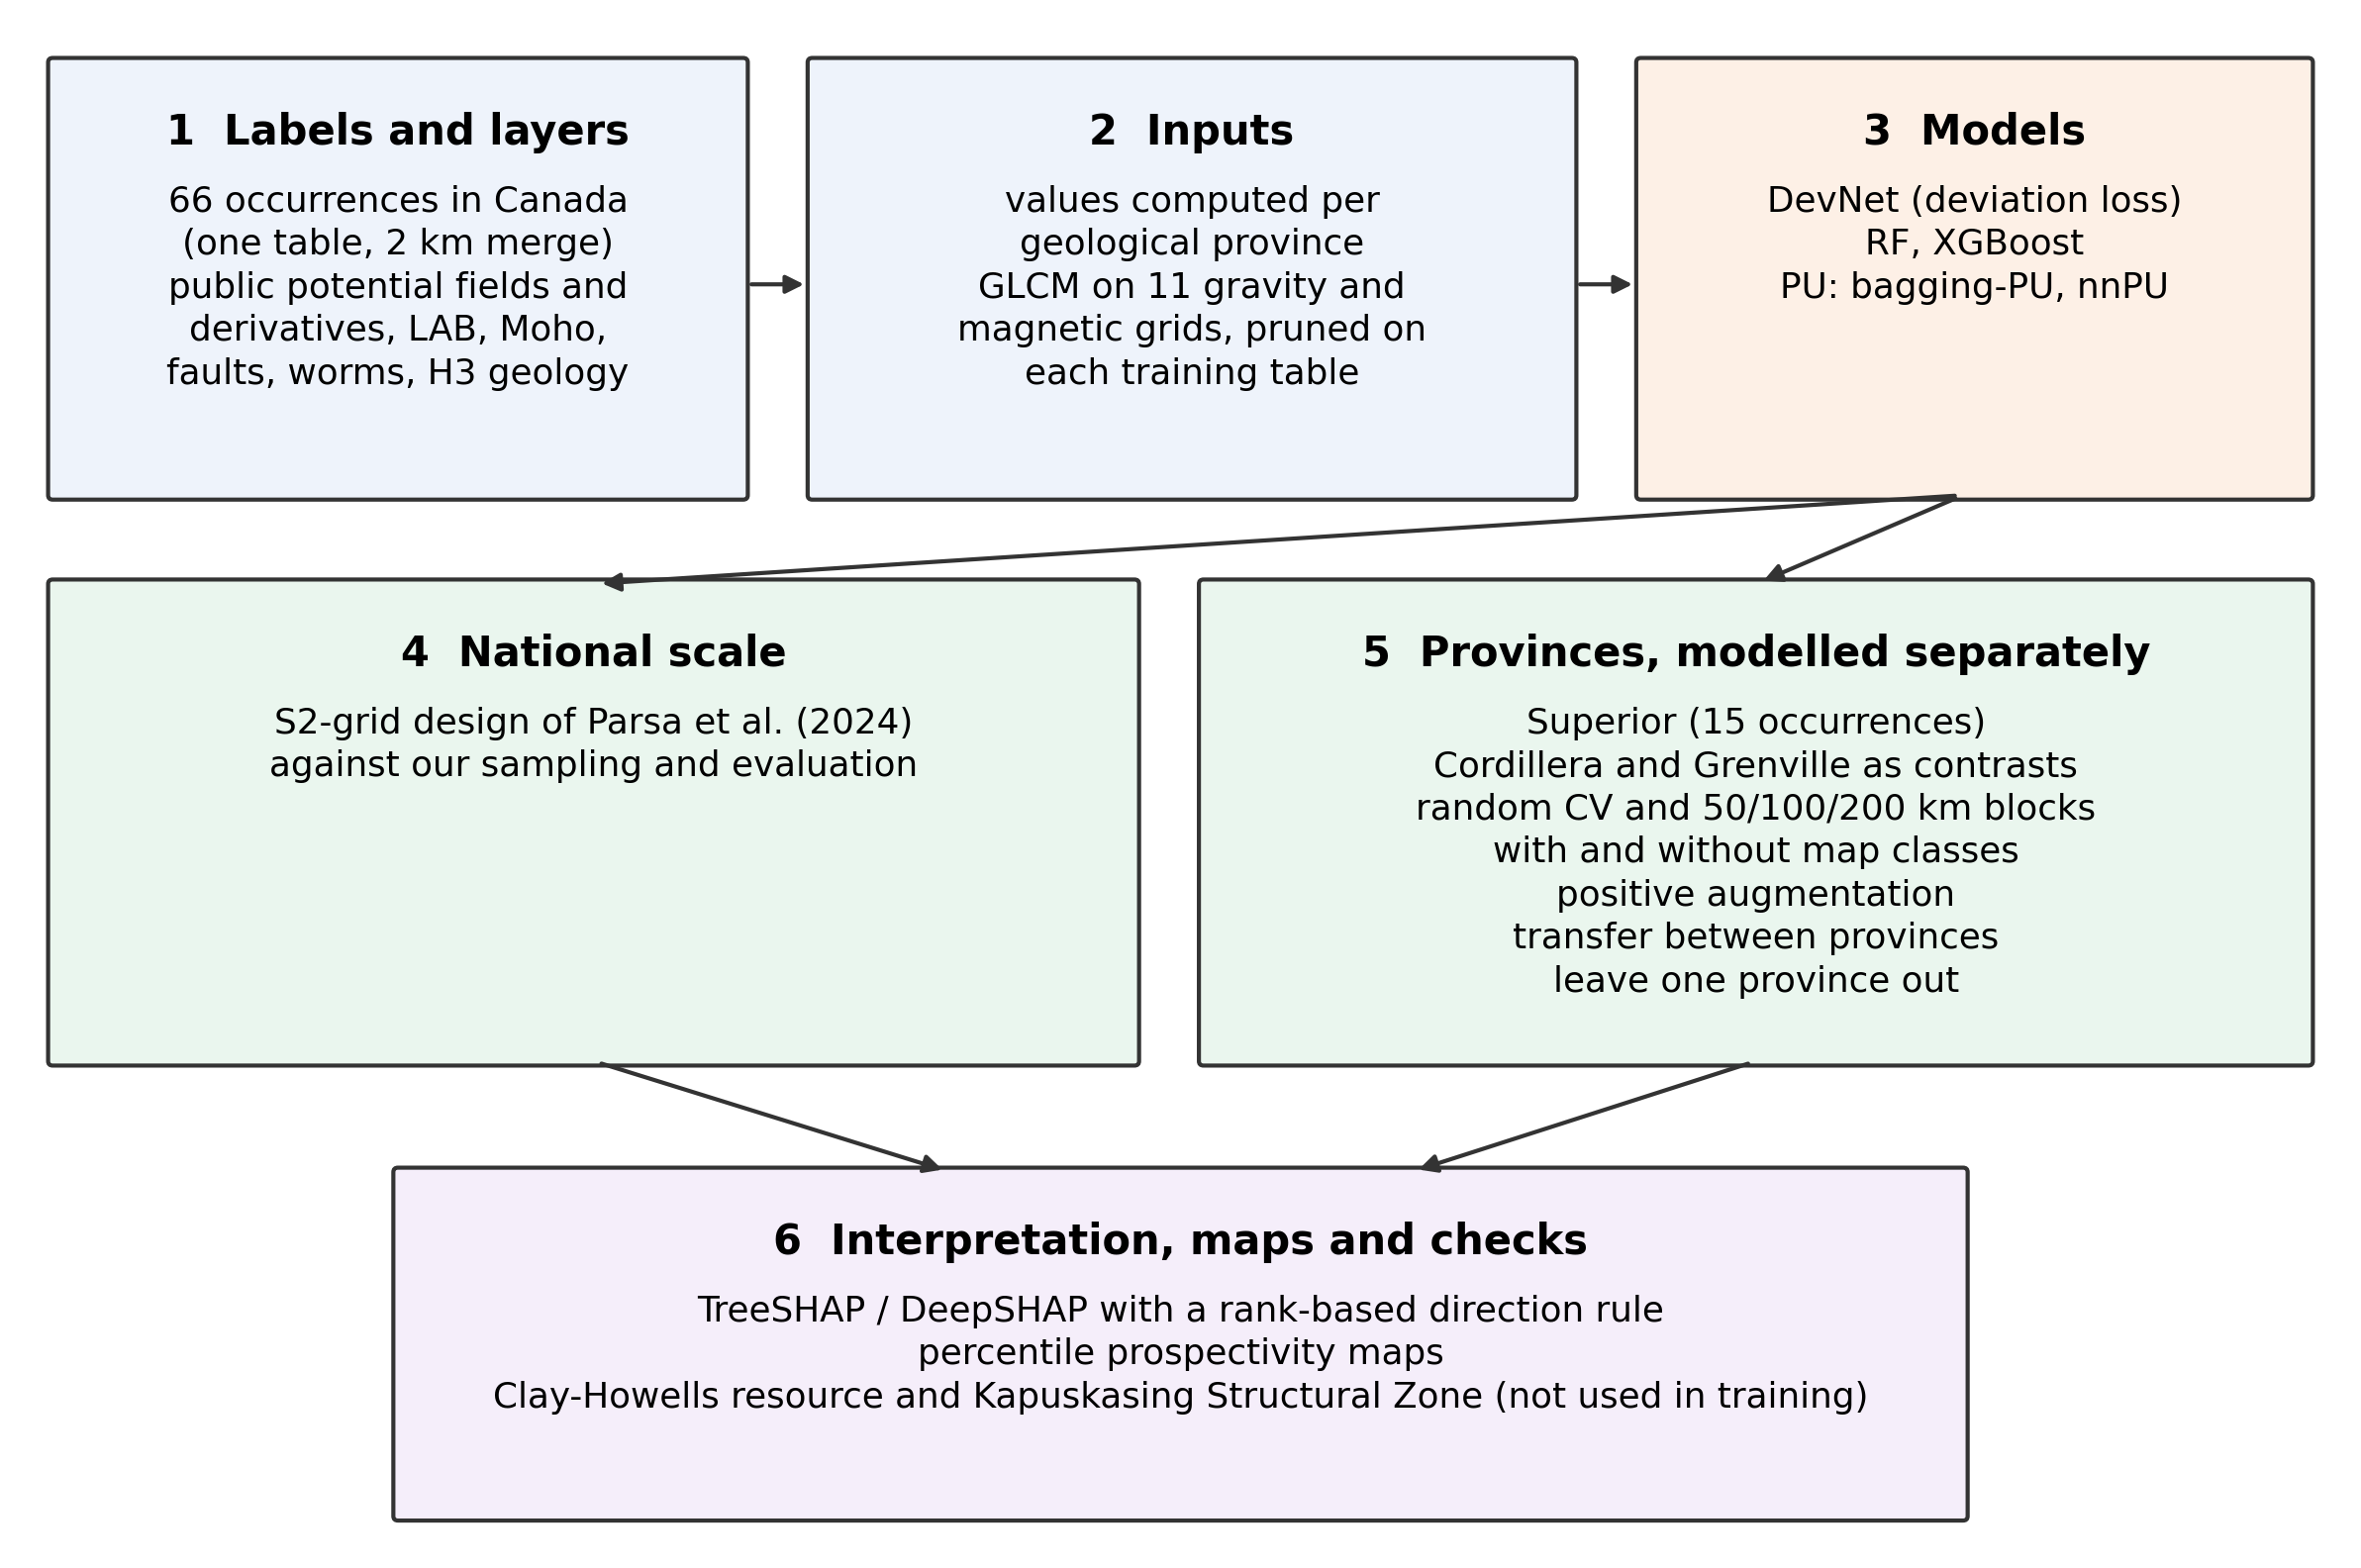
\includegraphics[width=\textwidth]{figures_r7/fig_workflow_r7.png}
\caption{Workflow. The national experiments motivate modelling the provinces separately. Within a comparison, all models are trained on the same positives and background and scored on the same folds; only the treatment of the background differs.}\label{fig:workflow}
\end{figure}

\subsection{National and provincial inputs}\label{sec:framework}

Three inputs depend on the extent of the area over which they are computed: raster values at the edge of a clip (a coarse pixel whose centre falls outside the buffered outline is nodata), the GLCM grey levels, which are quantised between the 2nd and 98th percentiles of the clipped raster, and the generalised geology map, which is built from the H3 cells in the outline's bounding box plus a margin. All three were computed per geological province, with the provincial rasters and bounding boxes for the study provinces, so that every national value equals the provincial one at the same point. Feature pruning (Section~\ref{sec:pruning}) and the H3 class list are applied to the table on which a model is trained: national models use the 71 inputs pruned on the national table, and the model of a province uses that province's inputs and network capacity, also when it is applied to another province.

\subsection{Feature pruning}\label{sec:pruning}

The candidate features include many collinear geophysical derivatives. Within each region, features were clustered hierarchically on $1-|\rho_{\mathrm{S}}|$ (Spearman correlation, average linkage) and cut at $|\rho_{\mathrm{S}}| = 0.7$, keeping one representative per cluster chosen by lowest missing rate and then highest variance \citep{Dormann2013}. The rule never sees labels and therefore cannot leak information across folds.

\subsection{Models}\label{sec:models}

All models see the same rows and differ only in how they treat the training background or in their loss.

\textbf{Random Forest} (RF; \citealp{Breiman2001}) is the discriminative baseline: positives versus training background labelled 0, 300 trees, $\sqrt{p}$ features per split, balanced class weights, inside a pipeline that fits median imputation and standardisation on the training fold only. With roughly 12 training positives against 5,000 background points, most held-out points receive a predicted probability of exactly zero, so the pooled AUC depends on which trees happen to vote for a given held-out occurrence. We therefore vary the RF seed across folds so that this variance enters the reported intervals.

\textbf{XGBoost} \citep{Chen2016} adds a gradient-boosted tree ensemble with parameters fixed in advance from a parallel national study of the same commodity rather than tuned here: 200 trees of depth 2, learning rate 0.1, row and column subsampling of 0.8, minimum child weight 3 and L2 and L1 penalties of 2 and 0.5. It is trained like RF, on median-imputed inputs with the positives up-weighted to balance the two classes.

\textbf{DevNet} \citep{Pang2019} maps each input vector $\mathbf{x}$ to a scalar score $\phi(\mathbf{x})$ through one hidden ReLU layer with dropout. The deviation $d(\mathbf{x}) = (\phi(\mathbf{x}) - \mu_R)/\sigma_R$ is measured against the mean and standard deviation of a fixed reference sample of 50,000 standard-normal draws, and the loss
\begin{equation}
L = (1-y)\,|d(\mathbf{x})| + y\,\max\{0,\, a - d(\mathbf{x})\}
\end{equation}
pulls unlabelled background ($y=0$) towards the reference and pushes positives ($y=1$) beyond a margin $a = 5$, the value of \citet{Pang2019} (Appendix~\ref{app:sensitivity}, Table~\ref{tab:margin}). Network capacity was set a priori by positive count (64 hidden units, dropout 0.3, weight decay $10^{-4}$ in Cordillera; 32, 0.4 and $10^{-3}$ in Superior and Grenville) rather than tuned, because a search over a few tens of positives fits noise. Training uses Adam \citep{Kingma2014} with weight decay, cosine learning-rate annealing over 300 steps and gradient clipping, and each fold score is the rank average of five restarts with different seeds.

Two design choices adapt DevNet to tabular evidence layers with very few positives. First, inputs are mapped to standard-normal marginals by a quantile transformation fitted on each training fold. Many evidence layers are strongly skewed (inverted distances concentrated near 0 or 1, long-tailed textures, 0/1 dummies), and unlike tree ensembles, which are invariant to monotone transformations, multilayer perceptrons are sensitive to such marginal distributions \citep{Gorishniy2021,Grinsztajn2022}. Second, each gradient step uses 16 positives (resampled with replacement) and 240 background rows. The deviation loss is meant to learn what the background looks like; with label-balanced batches of 16 + 16 rows, 300 steps would show each background row about once and each positive about 400 times, whereas background-heavy batches show each background row about 14 times while positive exposure is unchanged. Both choices were settled with diagnostic runs on these provinces using an earlier, coarser encoding of the geology; Appendix~\ref{app:sensitivity} repeats the ablation with the inputs used here.

\textbf{Bagging-PU} \citep{Mordelet2014} trains 200 fully grown decision trees, each on all training positives and an equal-sized bootstrap sample of the unlabelled background, and averages their outputs. It is the standard tree-based PU learner and the closest PU analogue of RF.

\textbf{nnPU} \citep{Kiryo2017} minimises the non-negative PU risk with the sigmoid loss, using exactly DevNet's network, quantile-normal inputs, optimiser, number of steps and five-restart ensemble, so that DevNet versus nnPU isolates the PU risk from the deviation loss. nnPU requires the class prior $\pi = P(y=1)$ in the unlabelled population; we use $\pi = 0.01$ (sensitivity in Appendix~\ref{app:full}, Table~\ref{tab:prior}). The calibration approach of \citet{Elkan2008} is not included because under its assumptions the calibrated output is a monotone transform of the positive-versus-background classifier, so its ranking, and every rank metric reported here, equals RF's.

\subsection{Evaluation protocol}\label{sec:protocol}

With three or four positives per validation fold, per-fold AUC is unstable and can be undefined, so out-of-fold scores are pooled \citep{BradleyAP1997}: each held-out point is scored once per repeat, scores are converted to within-fold percentile ranks so that folds are comparable, and a single AUC and average precision (AP) are computed over all folds. Pooling carries a small known negative bias in AUC \citep{Airola2019,Parker2007}. We emphasise AP because, at 0.5\% prevalence, it reflects the practical task of concentrating occurrences into a small search area, whereas AUC is dominated by the bulk of easily rejected background \citep{Saito2015}. Exploration efficiency is also shown as capture-rate curves: the share of held-out occurrences ranked within a given top fraction of the scored pool \citep{Chung2003,Agterberg2005}. Because the evaluation background is a random sample of the domain, this fraction approximates search area. Because unexplored background may host undiscovered occurrences, all metrics are conservative.

\textbf{Random cross-validation.} Repeated stratified 5-fold cross-validation with six repeats gives six pooled AUC and AP values per model, reported as the median and the 2.5--97.5 percentile interval over repeats (labelled 95\% interval). All models use identical splits, so they can be compared pairwise.

\textbf{Spatially blocked cross-validation.} Random folds can hold out an occurrence a few kilometres from a training occurrence. Following \citet{Roberts2017} and \citet{Valavi2019}, labelled points were assigned to square blocks of 50, 100 or 200~km side in Canada Atlas Lambert (EPSG:3978), whole blocks were held out together using stratified group 5-fold splitting (fewer folds if fewer blocks contain positives), and every training-background point falling inside a held-out block was removed from training for that fold. Each of six repeats uses a random offset of the block grid.

\textbf{Paired comparisons.} For each pair of models we average each point's out-of-fold rank over the six repeats and draw 5,000 stratified bootstrap resamples of positives and background \citep{Efron1993}, reporting the difference in AP and AUC with its 95\% percentile interval and the number of the six repeats in which the first model has the higher AP. With 12--27 positives these comparisons have little power, so we treat a difference as established only when it is consistent across repeats, block sizes and provinces.

\subsection{National-scale experiments}\label{sec:national-methods}

\textbf{Sampling and augmentation.} We rebuilt the national S2-grid design of \citet{Parsa2024} with the same geometry library on every level-12 S2 cell (about 4.5~km$^2$) whose centre lies in the national domain (1,616,693 cells), with the inputs extracted at the cell centres; the 66 occurrences fall in 66 cells. As in the original study, each occurrence cell was replaced by its four level-13 children, an equal number of negatives was drawn from the 5\% of cells with the lowest mean cosine similarity to the positives in min--max scaled feature space, and a random forest of 1,000 trees on min--max scaled inputs, the random-forest configuration of the original study, was evaluated by test AUC over 50 stratified 70/30 splits of the augmented labels. The original study's best model was a CNN; we keep the random forest because the elements examined here, the labels, the negatives and the split, determine how easy the test set is whatever the classifier. In our design the same forest, with balanced class weights, is trained on one label per occurrence cell against a random sample of 34,761 cells more than 10~km from any occurrence, and tested on the held-out 30\% of occurrence cells against a random 30\% of a disjoint sample of 20,855 cells, a realistic prevalence of about 0.3\%. To see which element of the original design drives its score, we also changed one element at a time: random instead of cosine-dissimilar negatives, and no augmentation.

\textbf{Transfer between provinces.} The model of province A (its inputs, capacity, occurrences and training background) scored the occurrences and evaluation background of province B, with six seeds; the diagonal, random cross-validation within A, is the provincial result. In leave-one-province-out validation a model trained on the national table without one province group (Superior, Cordillera, Grenville or the rest of Canada) scored that group. To describe the differences between provinces, a random forest (300 trees, 5-fold cross-validation) tried to tell the training background of two province groups apart, and the occurrences of two provinces; and the AUC of each input alone, for a province's occurrences against its evaluation background, gives the direction in which the input marks occurrences there.

\subsection{Synthetic positives}\label{sec:augmentation}

To test whether synthetic positives can compensate for label scarcity, each training fold's real positives were augmented with $m \times n_{\mathrm{pos}}$ synthetic positives ($m = 1, 3, 10$) before RF and DevNet were retrained; the held-out positives were always real. Three generators were compared, all fitted in the standardised feature space of the training fold only: Gaussian jitter of real positives ($\sigma = 0.1$ standard deviations); SMOTE-style interpolation between a positive and one of its three nearest positive neighbours \citep{Chawla2002}; and a tabular Wasserstein GAN with gradient penalty \citep[WGAN-GP;][]{Goodfellow2014,Arjovsky2017,Gulrajani2017} with an eight-dimensional latent input, two hidden layers of 64 units in generator and critic, five critic updates per generator update, gradient-penalty weight 10 and 2,000 generator updates, trained on the fold's 12 positives. Synthetic geology columns were snapped back to valid one-hot and 0/1 values. To see what the generators produce, each was also fitted to all 15 Superior positives and 150 samples were characterised by the distance to the nearest real positive divided by the median nearest-neighbour distance among real positives (a value near 0 indicates copying), by the share of samples whose nearest labelled neighbour is a positive rather than a background point, and by their DevNet score percentile.

\subsection{Interpretation and mapping}\label{sec:shap}

Production models were fitted to all positives and the training background of each region. SHAP values \citep{Lundberg2017} were computed with TreeSHAP for RF \citep{Lundberg2020} and DeepSHAP for DevNet on an explain set of all positives plus evaluation-background points (200 in total), with 100 training-background points as DevNet's reference sample; DevNet's SHAP values refer to its quantile-transformed inputs, which leaves the rank-based directions defined below unaffected. DevNet SHAP values were averaged over the five ensemble members. Importance is mean $|$SHAP$|$. The \emph{direction} of a feature's effect is the Spearman correlation between the feature's value and its SHAP value over the explain set (for one-hot dummies, the sign of the mean SHAP difference between presence and absence), with $|\rho| < 0.1$ reported as no clear direction. We do not use the sign of the mean SHAP value, which reflects where the explained points lie relative to the explainer's baseline rather than whether higher feature values raise the score: for RF with balanced class weights the TreeSHAP baseline is near 0.5 while nearly all explained points score near 0, so that rule would label every RF feature as ``higher $\rightarrow$ less prospective''. Prospectivity maps classify each model's scores on a 0.1$^\circ$ prediction grid into the top 1\%, 5\% and 10\%, because DevNet's anomaly score and RF's probability are not on a common scale. As an external check, the production models scored Clay-Howells, a drill-tested Fe--REE--Nb prospect with reported resources on the KSZ \citep{OGS2011} that is not among the training labels, at its recorded location.

%% ===================================================================
\section{Results}\label{sec:results}

\subsection{National scale}\label{sec:res-national}

\subsubsection{Sampling and augmentation in the S2-grid design}\label{sec:res-ladder}

Rebuilt on our national data, the design of \citet{Parsa2024} gives a test AUC of 1.000 (Table~\ref{tab:nat-design}), as high as the published 0.91--0.96 or higher. With one label per occurrence cell, random background and a realistic prevalence, the same forest reaches an AUC of 0.903 and an AP of 0.292. Each of the two elements of the original design suffices on its own for a near-perfect score. Splitting augmented children at random leaves a sibling of 97\% of the test positives in the training set, and with random negatives the AUC stays at 0.997; cosine-dissimilar negatives without any augmentation give 0.998, because the ground least similar to the occurrences is easy to reject. Such negatives also make a worse model: trained against them rather than against random negatives in an otherwise identical design, the forest's AP at realistic prevalence falls from 0.190 to 0.113.

\begin{table}[t]
\caption{The national S2-grid design of \citet{Parsa2024} and ours, with the same random forest (1,000 trees, min--max inputs): mean test AUC and AP over 50 stratified 70/30 splits. Test set: occurrence share among the test points.}\label{tab:nat-design}
\scriptsize
\setlength{\tabcolsep}{2.5pt}
\begin{tabular*}{\textwidth}{@{\extracolsep\fill}>{\raggedright\arraybackslash}p{1.8cm}>{\raggedright\arraybackslash}p{2.6cm}>{\raggedright\arraybackslash}p{2.7cm}>{\raggedright\arraybackslash}p{1.9cm}>{\raggedright\arraybackslash}p{1.4cm}cc}
\toprule
Design & Positive labels & Negatives & Split & Test set & AUC & AP \\
\midrule
Parsa et al. (2024) & four L13 children per occurrence cell (264) & 264 cells from the 5\% least cosine-similar & child labels, random 70/30 & balanced (50\%) & 1.000 & 1.000 \\
This study & one per occurrence cell (66) & 34,761 random cells $>$10~km from occurrences & occurrence cells, random 70/30 & realistic (0.3\%) & 0.903 & 0.292 \\
\botrule
\end{tabular*}
\end{table}

\subsubsection{Transferability between provinces}\label{sec:res-transfer}

A province's model does not predict another province (Fig.~\ref{fig:transfer}). Within each province, random cross-validation gives an AP of 0.13--0.47 (nnPU excluded); applied to another province, the tree ensembles reach 0.004--0.016, about the random-ranking values of 0.004--0.009, and in 18 of the 30 model--province pairs the AUC is below 0.5: the model ranks the other province's occurrences below its background. The exceptions are DevNet, XGBoost and nnPU trained in Cordillera and bagging-PU trained in Grenville, applied to Superior: they reach AUCs of 0.73--0.75 but APs of only 0.013--0.086, against 0.005 for a random ranking. Leaving a province out of a national model gives the same picture: held-out Grenville is ranked close to chance (AUC 0.36--0.67, AP $\leq 0.037$, against 0.004 for a random ranking), and held-out Superior reaches an AP of at most 0.051 (random ranking 0.005).

The provinces are distinct domains in the inputs. A random forest separates the training background of any two province groups with an AUC of 0.999--1.000, and the occurrences of Superior, Cordillera and Grenville from one another with 0.99--1.00. Several inputs mark occurrences in opposite directions in different provinces. Taken alone, LAB depth separates Superior occurrences from their background with an AUC of 0.22 (shallower LAB at occurrences) but Cordilleran ones with 0.67 (deeper), Moho depth with 0.35 and 0.78, and distance to regional greenstone with 0.23 and 0.63; deep-source magnetics marks Cordilleran and Grenville occurrences in opposite directions (0.25 and 0.81). The rest of the study therefore models each province separately.

\begin{figure}[t]
\centering
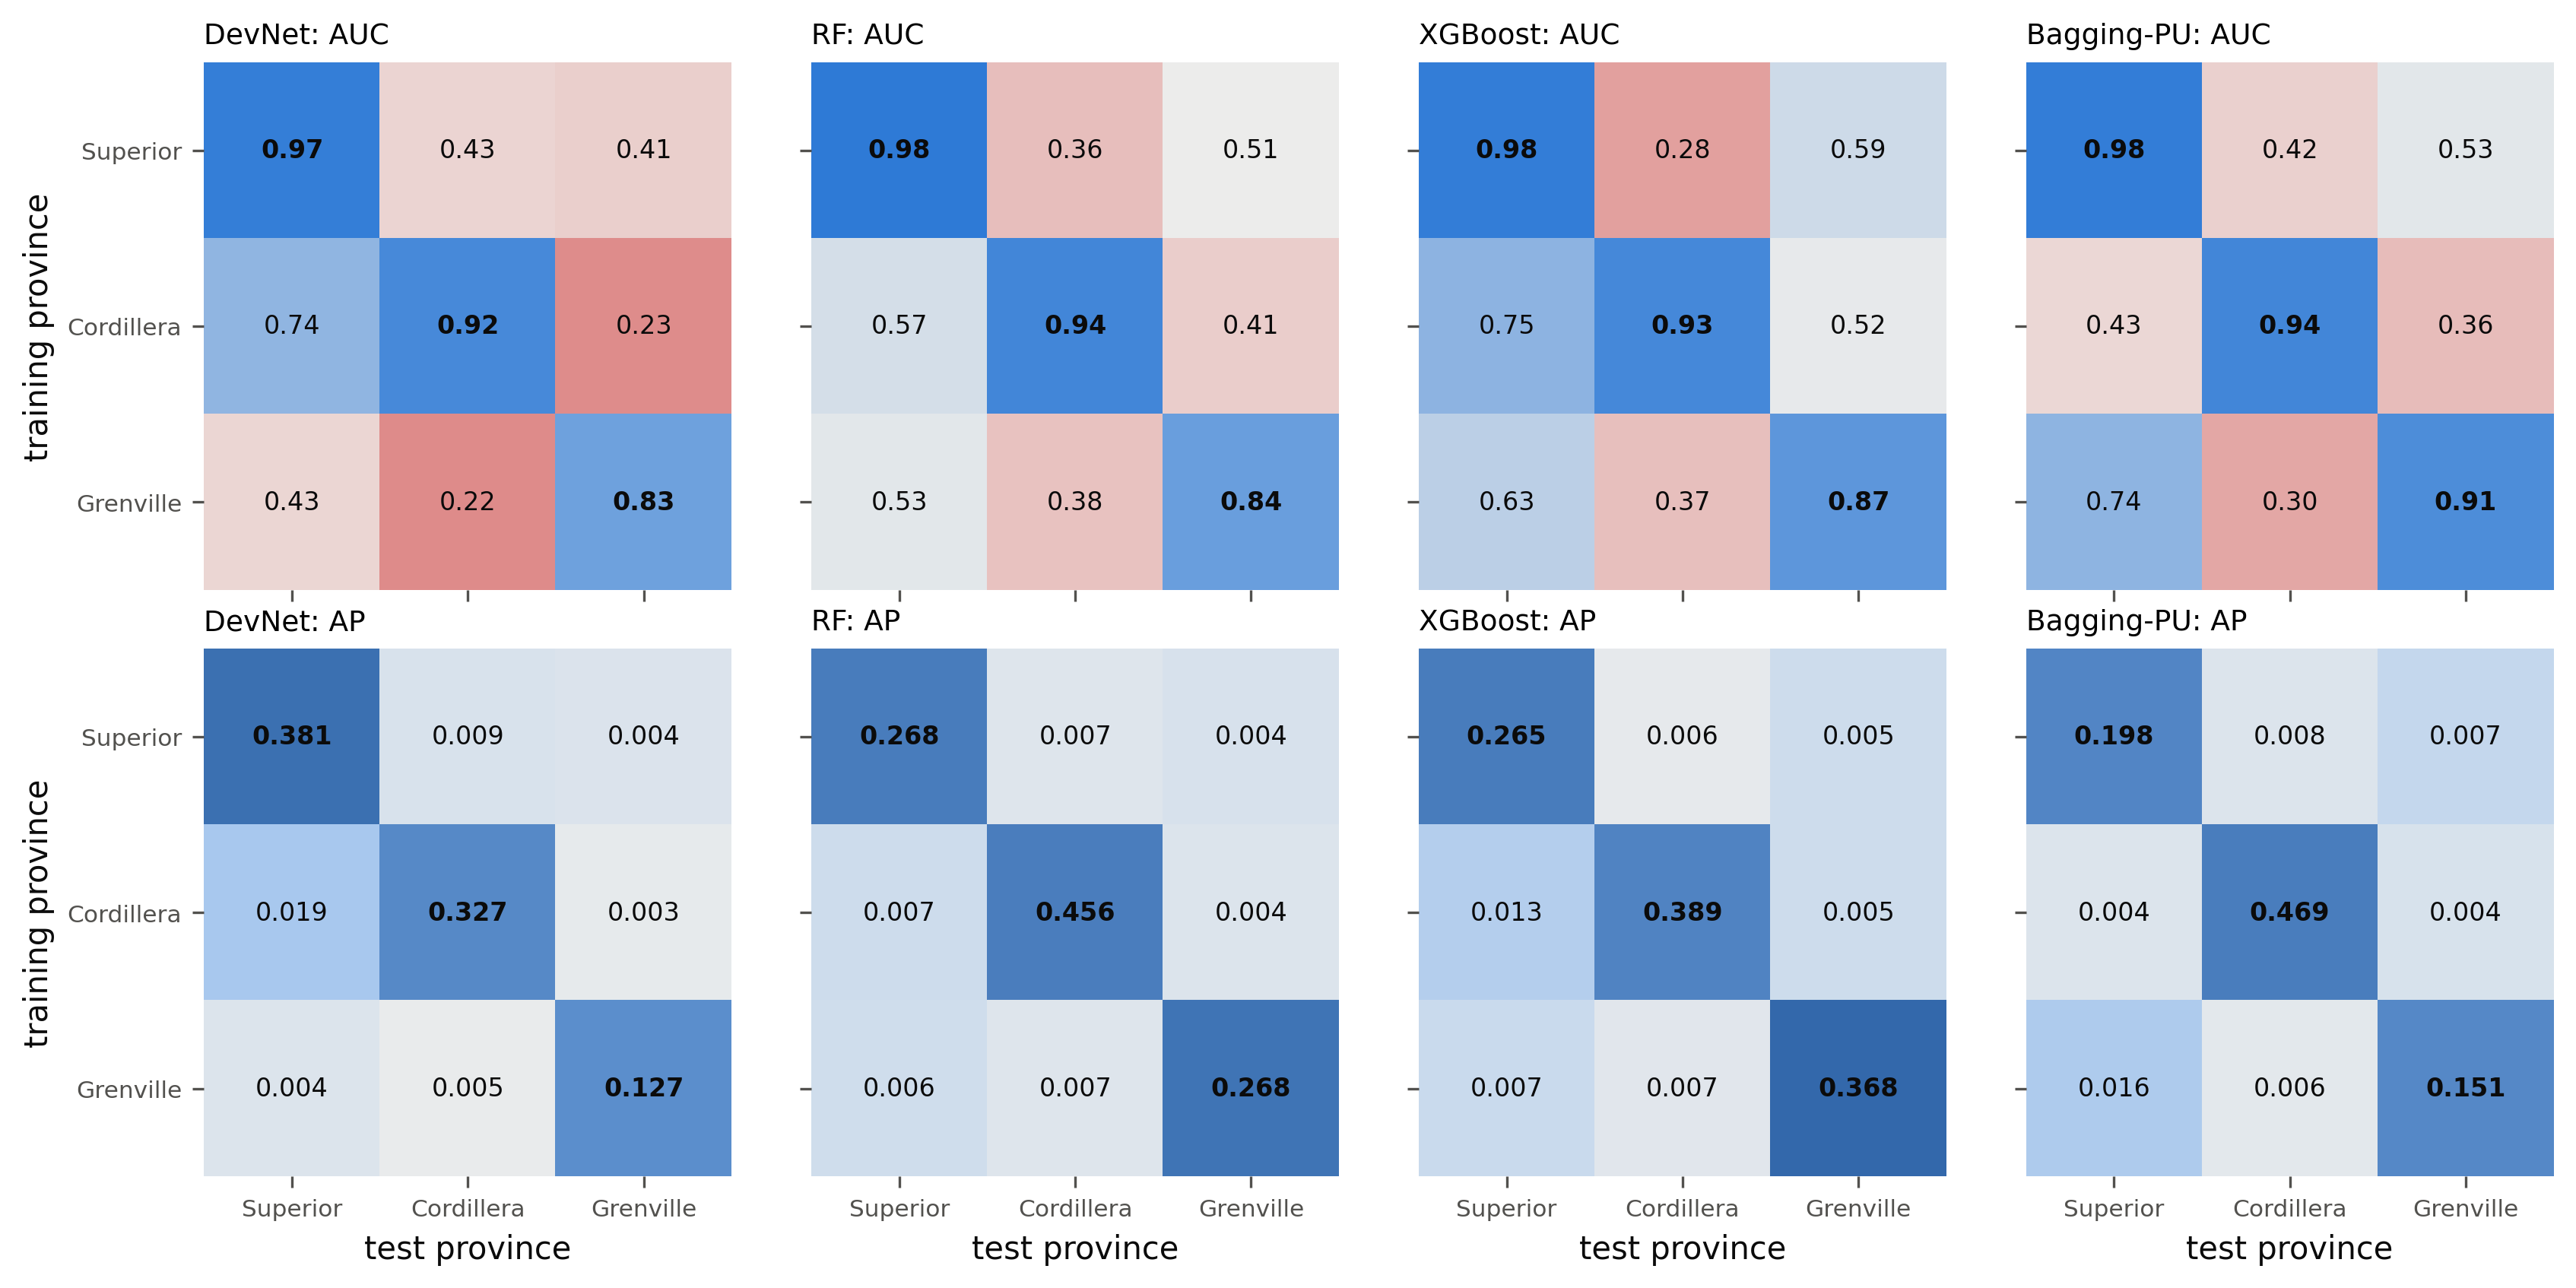
\includegraphics[width=\textwidth]{figures_r7/fig_transfer_r5.png}
\caption{Transfer between provinces. Top: AUC; bottom: AP, coloured by AP divided by the test province's prevalence (log scale). Rows: province whose model (inputs, capacity, occurrences, training background) is applied; columns: province whose occurrences and evaluation background are scored (median of six seeds). The diagonal is random cross-validation within the province (Table~\ref{tab:benchmark}).}\label{fig:transfer}
\end{figure}

\subsection{Provincial models}\label{sec:res-provinces}

\subsubsection{Model comparison under random cross-validation}\label{sec:res-random}

In Superior all models except nnPU rank held-out occurrences far above chance (Table~\ref{tab:benchmark}): AP is 0.20--0.38 against a random-ranking value of 0.005, and AUC is 0.97--0.99. DevNet has the highest median AP (0.381) and RF the highest AUC (0.985). DevNet's AP exceeds RF's, XGBoost's (0.265), bagging-PU's and nnPU's in all six repeated splits, by 0.18--0.30 on repeat-averaged ranks. nnPU, which shares DevNet's network and inputs, reaches an AP of only 0.159 and an AUC of 0.842.

The contrasting regions behave differently. In Cordillera, bagging-PU and RF lead (AP 0.469 and 0.456), and DevNet (0.327; lower than RF in all six repeats) and XGBoost (0.389) trail. In Grenville all models are weak; XGBoost leads (0.368), followed by RF (0.268), both ahead of DevNet (0.127) in all six repeats. nnPU fails in both provinces (AUC 0.58--0.61). That Superior is the best-predicted of the three provinces agrees with the province-level success rates of \citet{Parsa2024}.

\begin{table}[t]
\caption{Pooled out-of-fold AUC and AP (median and 95\% interval over six repeated 5-fold random splits). Bold: best of the five models in each region.}\label{tab:benchmark}
\footnotesize
\begin{tabular*}{\textwidth}{@{\extracolsep\fill}llcc}
\toprule
Region ($n_{\mathrm{pos}}$) & Model & AUC & AP \\
\midrule
\multirow{5}{*}{Superior (15)} & DevNet & 0.972 & \textbf{0.381} [0.347, 0.452] \\
 & RF & \textbf{0.985} & 0.268 [0.202, 0.314] \\
 & XGBoost & 0.976 & 0.265 [0.243, 0.298] \\
 & Bagging-PU & 0.976 & 0.198 [0.163, 0.219] \\
 & nnPU & 0.842 & 0.159 [0.096, 0.210] \\
\midrule
\multirow{5}{*}{Cordillera (27)} & DevNet & 0.925 & 0.327 [0.263, 0.353] \\
 & RF & 0.936 & 0.456 [0.428, 0.548] \\
 & XGBoost & 0.926 & 0.389 [0.357, 0.448] \\
 & Bagging-PU & \textbf{0.937} & \textbf{0.469} [0.356, 0.485] \\
 & nnPU & 0.575 & 0.023 [0.017, 0.037] \\
\midrule
\multirow{5}{*}{Grenville (12)} & DevNet & 0.826 & 0.127 [0.060, 0.168] \\
 & RF & 0.836 & 0.268 [0.202, 0.320] \\
 & XGBoost & 0.870 & \textbf{0.368} [0.216, 0.429] \\
 & Bagging-PU & \textbf{0.909} & 0.151 [0.133, 0.197] \\
 & nnPU & 0.609 & 0.009 [0.008, 0.010] \\
\botrule
\end{tabular*}
\end{table}

\subsubsection{Spatially blocked cross-validation}\label{sec:res-spatial}

Holding out whole blocks widens the gap between DevNet and the tree-based and PU learners in Superior (Fig.~\ref{fig:spatial}; Table~\ref{tab:spatial}). DevNet's AP is 0.371, 0.345 and 0.221 with 50, 100 and 200~km blocks. RF's falls from 0.268 under random splits to 0.165, 0.129 and 0.087, XGBoost's from 0.265 to 0.177, 0.119 and 0.098, and bagging-PU's to 0.133, 0.076 and 0.072. DevNet has the higher AP than RF, XGBoost and bagging-PU in all six repeats at every block size, and than nnPU in 16 of the 18, by $+0.23$ to $+0.31$ against RF, $+0.21$ to $+0.33$ against XGBoost, $+0.25$ to $+0.39$ against bagging-PU and $+0.13$ to $+0.30$ against nnPU. With 15 occurrences, however, the 95\% intervals of the differences from RF reach down to 0.03--0.06, so the margin over RF is consistent but its size is uncertain. AUC differs less between models (Appendix~\ref{app:full}, Table~\ref{tab:spatial-auc}): RF has the highest AUC with 50~km blocks (0.976 against 0.969 for DevNet), and DevNet with 100 and 200~km blocks (0.928 and 0.886). Under 50 and 100~km blocks the occurrences that DevNet ranks lowest are Kapuskasing and Nemegosenda Lake, on the KSZ.

Capture-rate curves (Fig.~\ref{fig:capture}) show where the AP differences arise. Under random splits DevNet and RF capture about half of the held-out occurrences in the top 1\% of the ranked pool (53\% and 50\%), and by the top 10\% RF captures all of them, bagging-PU 97\% and DevNet 93\%. With 50 and 100~km blocks DevNet keeps most of its top-1\% capture (53\% and 43\%) and captures 93\% and 87\% by the top 10\%, whereas RF captures 40\% and 27\% in the top 1\% (100\% and 77\% by the top 10\%) and bagging-PU 30\% and 23\% (90\% and 70\%). With 200~km blocks every model captures 40\% or less in the top 1\%, and by the top 10\% DevNet and bagging-PU (70\%) slightly exceed RF (63\%).

In Cordillera every model degrades sharply under blocking (AP $\leq 0.13$ at 50~km and $\leq 0.07$ at 100--200~km), and in Grenville AP approaches the random-ranking value ($\leq 0.010$ at 100--200~km). In these regions no difference between models is of practical size: their random-split skill owes much to spatial proximity between training and test occurrences (Section~\ref{sec:disc-provinces}).

\begin{figure}[t]
\centering
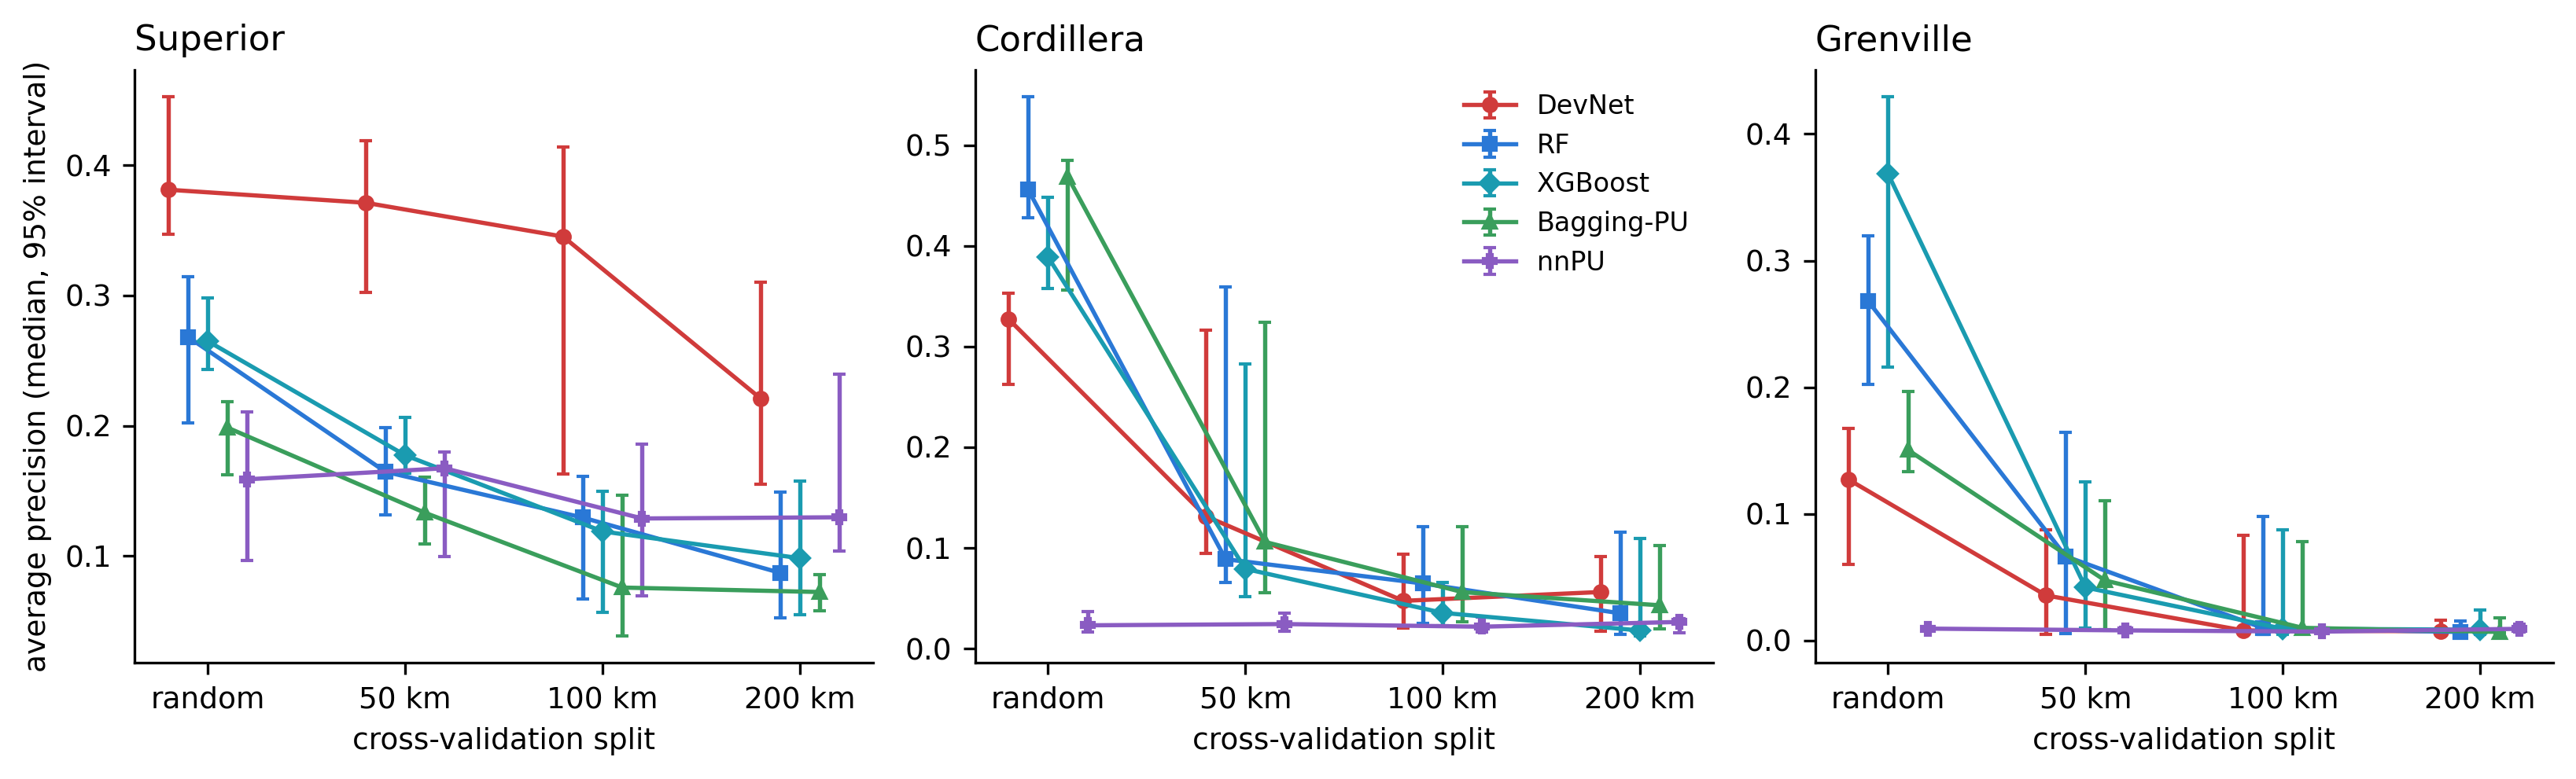
\includegraphics[width=\textwidth]{figures_r7/fig_spatial_cv_r5.png}
\caption{Average precision under random and spatially blocked cross-validation (median and 95\% interval over six repeats). The random-ranking AP is 0.005 (Superior), 0.009 (Cordillera) and 0.004 (Grenville).}\label{fig:spatial}
\end{figure}

\begin{figure}[t]
\centering
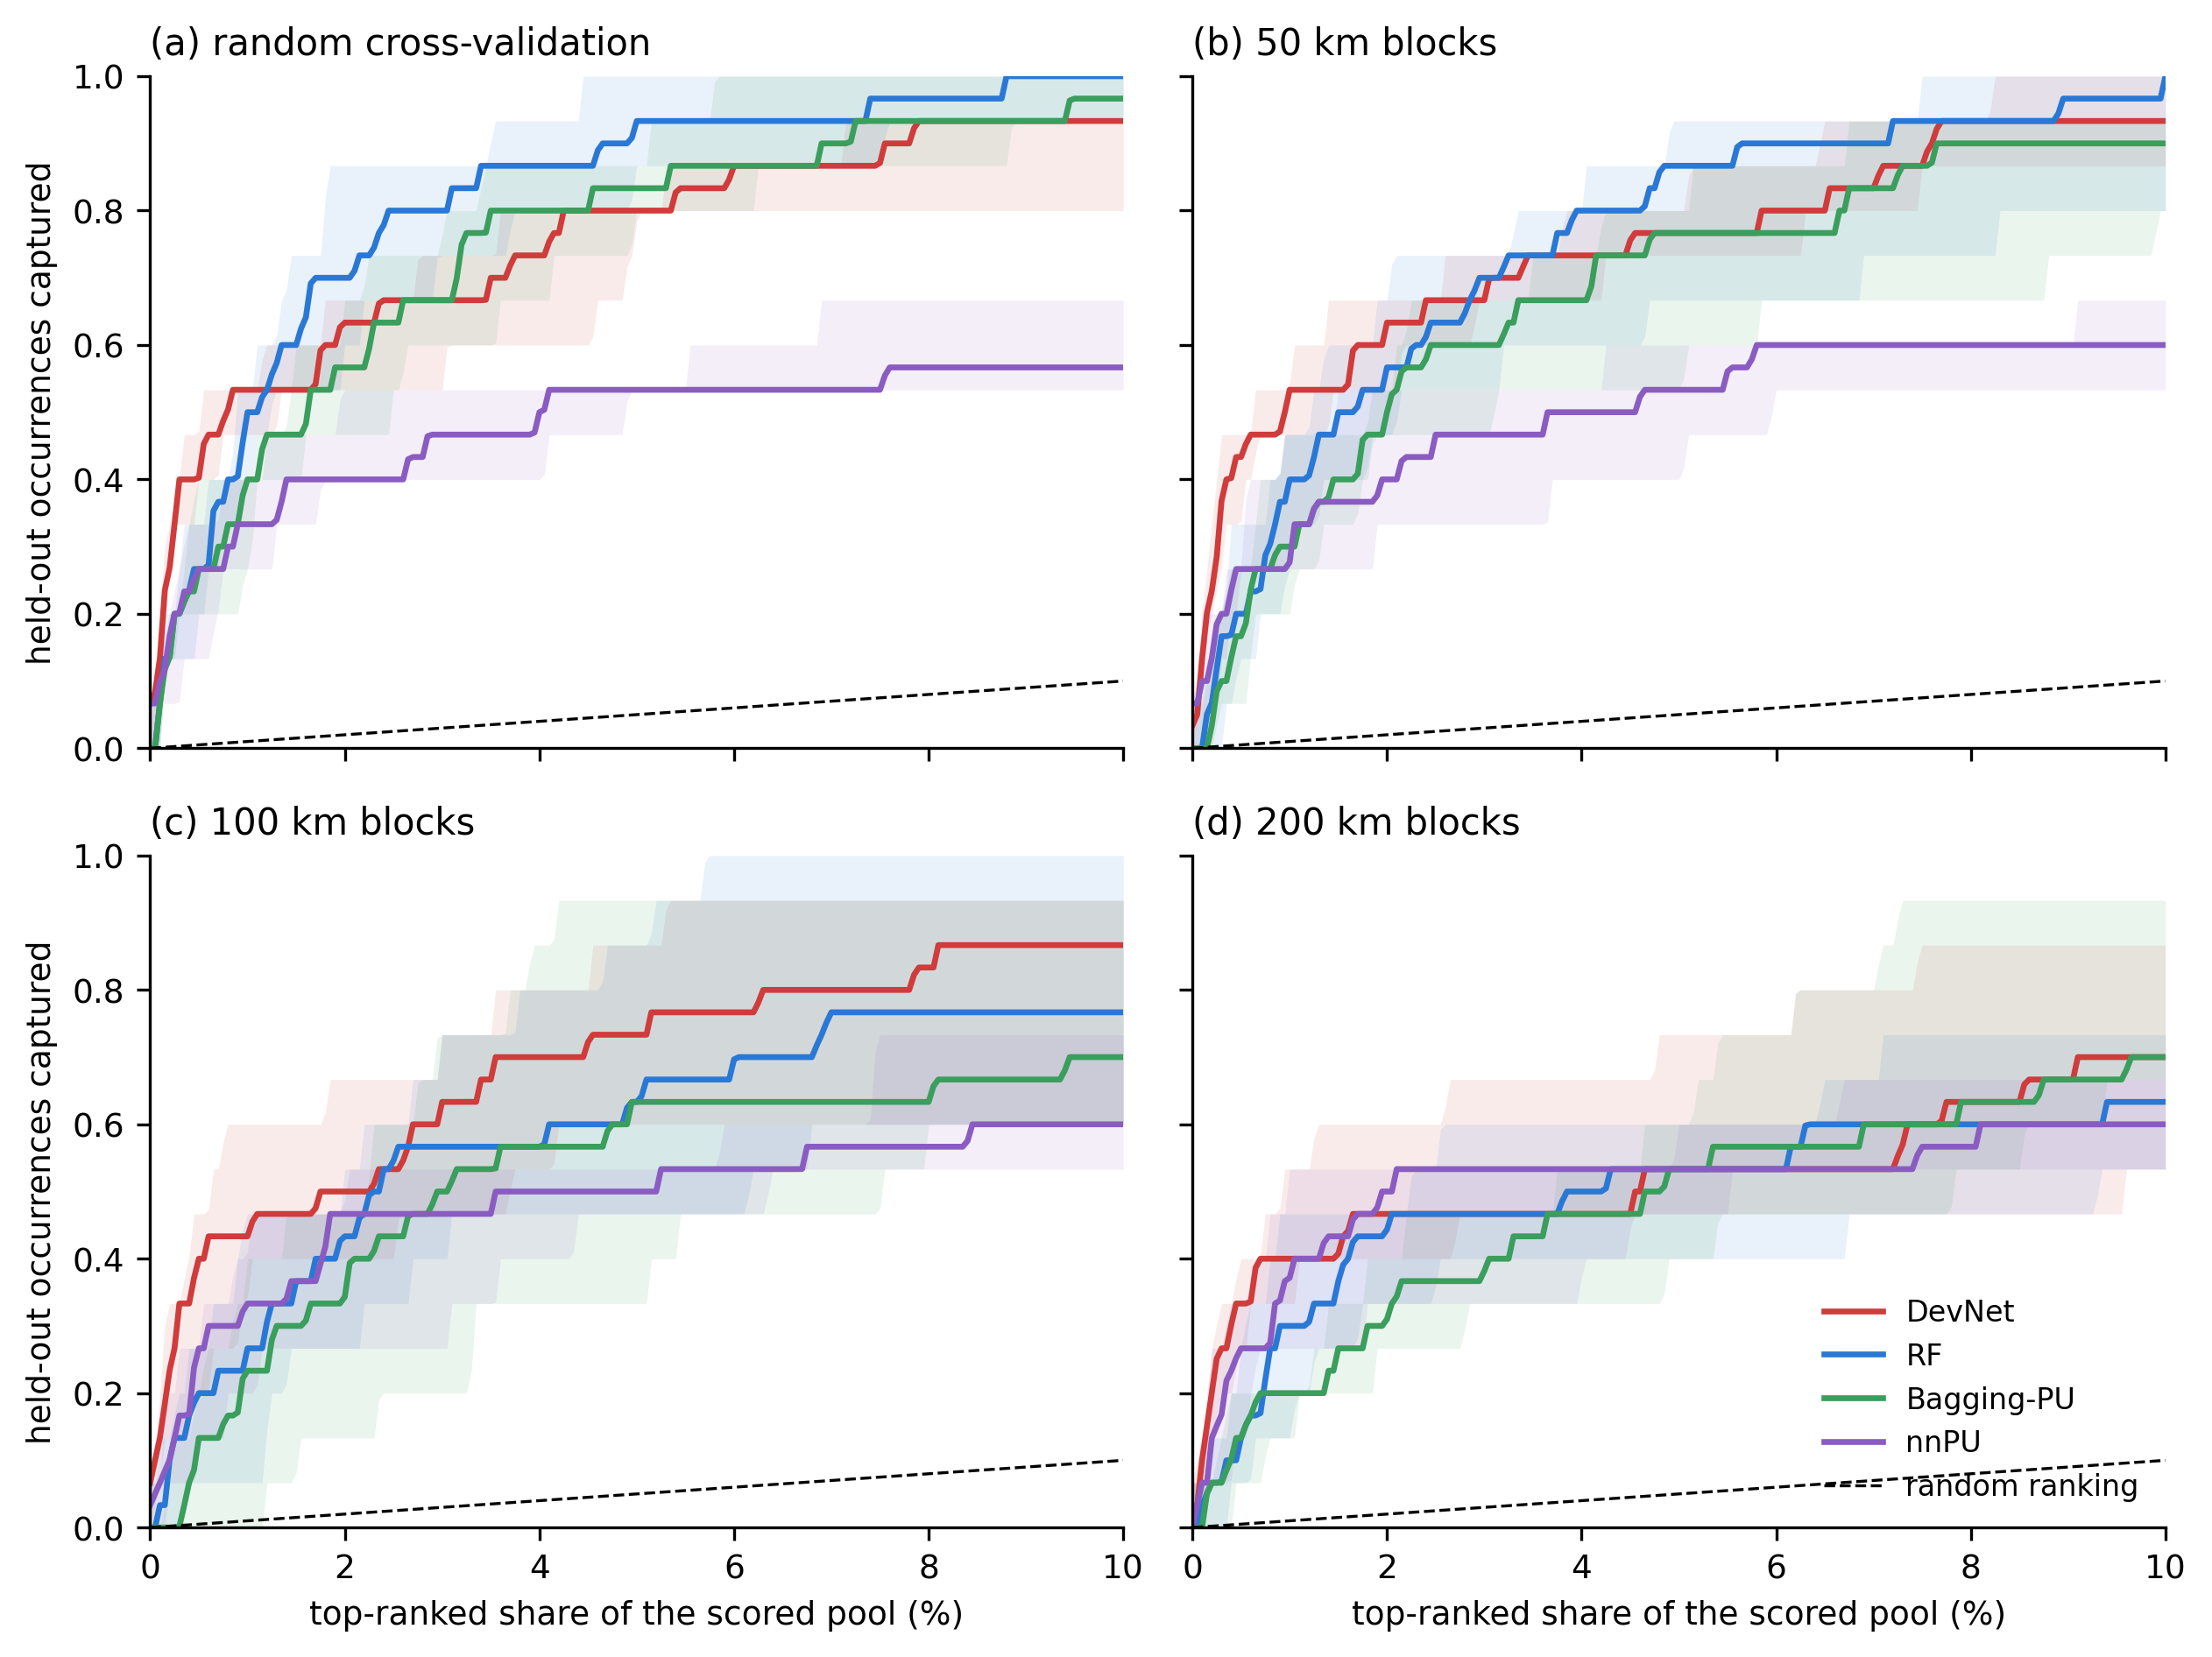
\includegraphics[width=0.92\textwidth]{figures_r7/fig_capture_superior_r4.png}
\caption{Superior capture-rate curves: share of held-out occurrences ranked within the top fraction of the scored pool (a proxy for search area) under (a) random cross-validation and (b) 50~km, (c) 100~km and (d) 200~km spatial blocks. Lines: median over six repeats; bands: range. Dashed: random ranking.}\label{fig:capture}
\end{figure}

\begin{table}[t]
\caption{Average precision (median over six repeats) under random and spatially blocked cross-validation. Bold: highest AP in each row. AUC for the same runs is given in Appendix~\ref{app:full} (Table~\ref{tab:spatial-auc}).}\label{tab:spatial}
\footnotesize
\setlength{\tabcolsep}{3pt}
\begin{tabular*}{\textwidth}{@{\extracolsep\fill}llccccc}
\toprule
Region & Split & DevNet & RF & XGBoost & Bagging-PU & nnPU \\
\midrule
\multirow{4}{*}{Superior} & random & \textbf{0.381} & 0.268 & 0.265 & 0.198 & 0.159 \\
 & 50 km & \textbf{0.371} & 0.165 & 0.177 & 0.133 & 0.167 \\
 & 100 km & \textbf{0.345} & 0.129 & 0.119 & 0.076 & 0.129 \\
 & 200 km & \textbf{0.221} & 0.087 & 0.098 & 0.072 & 0.130 \\
\midrule
\multirow{4}{*}{Cordillera} & random & 0.327 & 0.456 & 0.389 & \textbf{0.469} & 0.023 \\
 & 50 km & \textbf{0.131} & 0.089 & 0.079 & 0.106 & 0.024 \\
 & 100 km & 0.048 & \textbf{0.065} & 0.036 & 0.056 & 0.022 \\
 & 200 km & \textbf{0.056} & 0.035 & 0.018 & 0.043 & 0.027 \\
\midrule
\multirow{4}{*}{Grenville} & random & 0.127 & 0.268 & \textbf{0.368} & 0.151 & 0.009 \\
 & 50 km & 0.036 & \textbf{0.067} & 0.042 & 0.047 & 0.008 \\
 & 100 km & 0.008 & 0.010 & 0.009 & \textbf{0.010} & 0.007 \\
 & 200 km & 0.007 & 0.007 & 0.009 & 0.007 & \textbf{0.009} \\
\botrule
\end{tabular*}
\end{table}

\subsubsection{Contribution of geological map classes}\label{sec:res-featuresets}

A single map class carries much of the skill in Superior. Removing the alkalic-intrusion column lowers DevNet's AP to 0.346, 0.260, 0.177 and 0.137 under random splits and 50, 100 and 200~km blocks, and RF's to 0.194, 0.126, 0.065 and 0.067: this one class, which covers 6 of the 15 Superior occurrences and 0.5\% of the background, accounts for 30--49\% of DevNet's spatially blocked AP. DevNet without it still has a higher AP than RF with it at every block size. Withholding all point-level map classes costs DevNet and RF about half or more of their AP: DevNet's falls to 0.159 under random splits and 0.123, 0.081 and 0.075 under blocks, RF's to 0.146 and 0.084, 0.044 and 0.050. Without map classes DevNet still has the highest AP under every block size, ahead of XGBoost (0.105, 0.050 and 0.062) and bagging-PU (0.102, 0.058 and 0.066), while XGBoost and bagging-PU lead under random splits (0.175 and 0.174) and nnPU fails (AP 0.009).

\subsubsection{Synthetic positives}\label{sec:res-augmentation}

The generators behave very differently (Table~\ref{tab:aug-diag}; Appendix~\ref{app:aug-spatial}, Fig.~\ref{fig:aug-pca}). Jitter and SMOTE samples lie close to the real positives (median nearest-neighbour ratio 0.11 and 0.24) and almost all have a real positive as their nearest labelled neighbour (100\% and 99\%): they are near-copies of the training occurrences. WGAN-GP samples are as far from the real positives as the real positives are from one another (ratio 0.97), but for 37\% of them the nearest labelled point is a background point: with 15 training points the generator spreads probability mass into background-like parts of feature space. All three sets of samples receive high DevNet scores (median percentile 0.98).

The folds are identical with and without augmentation (Table~\ref{tab:augmentation}; Fig.~\ref{fig:aug-perf}). For DevNet every generator raises the median AP somewhat (with augmentation its AP lies between 0.408 and 0.432, against 0.381 without), but not consistently: augmented DevNet has the higher AP in only two to five of the six repeated splits. For RF, jitter changes the AP from 0.268 to 0.264--0.310, SMOTE lowers it (0.198--0.236) and WGAN-GP raises it (0.278--0.327). The best augmented RF (WGAN-GP $10\times$, AP 0.327) remains below DevNet without augmentation (0.381). Under spatial blocking (Appendix~\ref{app:aug-spatial}, Table~\ref{tab:aug-spatial}) WGAN-GP raises RF's AP with 100~km blocks from 0.129 to 0.135--0.191 and with 200~km blocks from 0.087 to 0.122--0.132, still well below unaugmented DevNet (0.345 and 0.221), whereas jitter and SMOTE change it little (0.110--0.139 and 0.077--0.096). DevNet's AP changes little with 100~km blocks (0.308--0.341 against 0.343) and varies between 0.200 and 0.258 with 200~km blocks (against 0.216).

\begin{figure}[t]
\centering
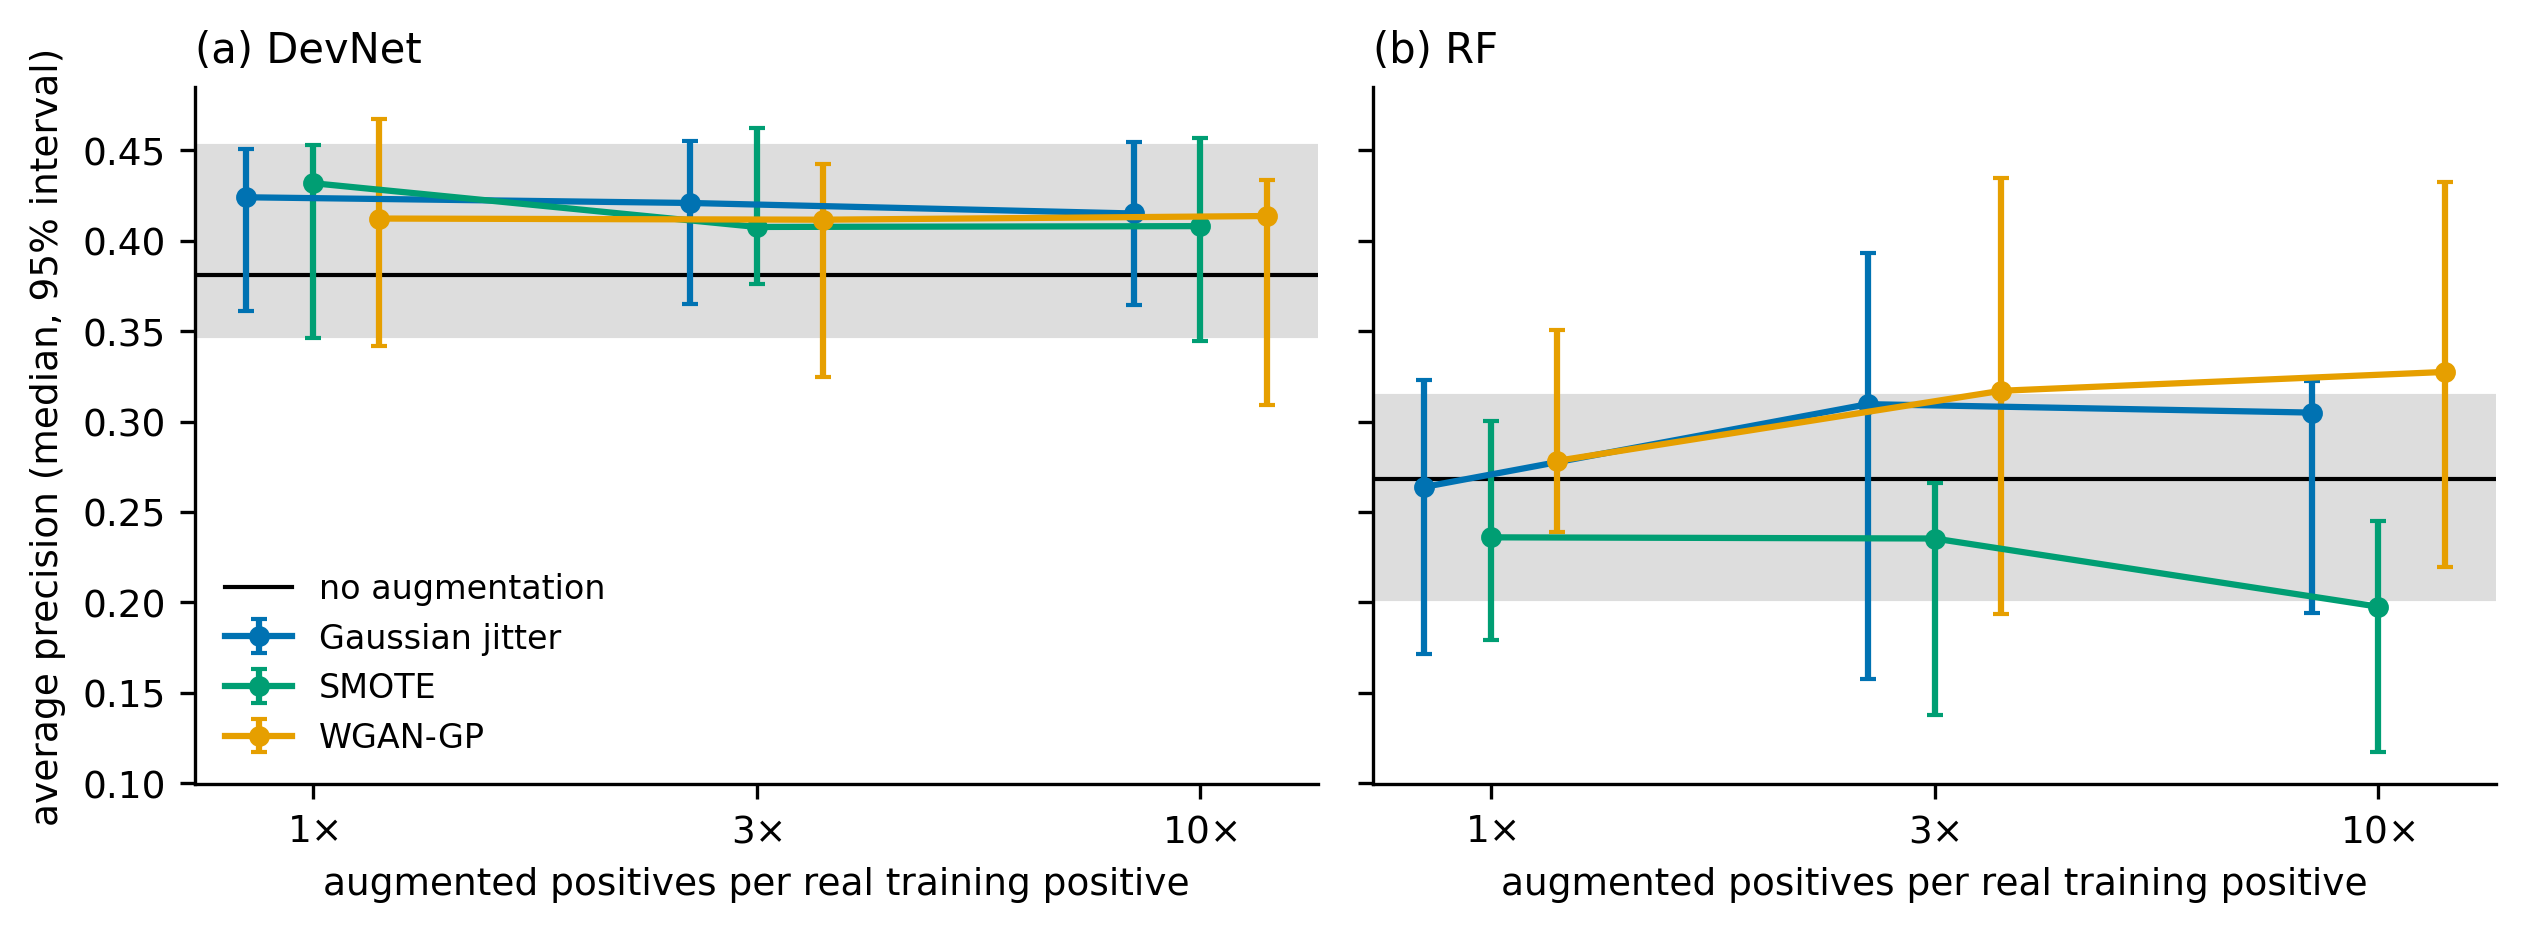
\includegraphics[width=\textwidth]{figures_r7/fig_augmentation_performance_r4.png}
\caption{Superior average precision with fold-safe synthetic positives, by generator and number of synthetic positives per real training positive. Line and grey band: no augmentation (median and 95\% interval).}\label{fig:aug-perf}
\end{figure}

\begin{table}[t]
\caption{Fold-safe positive augmentation, Superior (random cross-validation, identical folds; held-out positives always real): AUC and AP (median and 95\% interval over six repeats).}\label{tab:augmentation}
\footnotesize
\begin{tabular*}{0.8\textwidth}{@{\extracolsep\fill}lllcc}
\toprule
Model & Generator & $m$ & AUC & AP \\
\midrule
\multirow{10}{*}{DevNet} & none & -- & 0.972 & 0.381 [0.347, 0.452] \\
 & Gaussian jitter & 1$\times$ & 0.966 & 0.424 [0.361, 0.451] \\
 & Gaussian jitter & 3$\times$ & 0.969 & 0.421 [0.365, 0.455] \\
 & Gaussian jitter & 10$\times$ & 0.971 & 0.415 [0.364, 0.455] \\
 & SMOTE & 1$\times$ & 0.973 & 0.432 [0.346, 0.453] \\
 & SMOTE & 3$\times$ & 0.975 & 0.408 [0.376, 0.462] \\
 & SMOTE & 10$\times$ & 0.970 & 0.408 [0.344, 0.457] \\
 & WGAN-GP & 1$\times$ & 0.973 & 0.412 [0.342, 0.467] \\
 & WGAN-GP & 3$\times$ & 0.968 & 0.412 [0.325, 0.442] \\
 & WGAN-GP & 10$\times$ & 0.960 & 0.414 [0.309, 0.433] \\
\midrule
\multirow{10}{*}{RF} & none & -- & 0.985 & 0.268 [0.202, 0.314] \\
 & Gaussian jitter & 1$\times$ & 0.964 & 0.264 [0.171, 0.323] \\
 & Gaussian jitter & 3$\times$ & 0.983 & 0.310 [0.158, 0.393] \\
 & Gaussian jitter & 10$\times$ & 0.980 & 0.305 [0.194, 0.323] \\
 & SMOTE & 1$\times$ & 0.981 & 0.236 [0.179, 0.300] \\
 & SMOTE & 3$\times$ & 0.983 & 0.235 [0.138, 0.266] \\
 & SMOTE & 10$\times$ & 0.980 & 0.198 [0.117, 0.245] \\
 & WGAN-GP & 1$\times$ & 0.984 & 0.278 [0.239, 0.351] \\
 & WGAN-GP & 3$\times$ & 0.983 & 0.317 [0.193, 0.435] \\
 & WGAN-GP & 10$\times$ & 0.984 & 0.327 [0.219, 0.433] \\
\botrule
\end{tabular*}
\end{table}

\begin{table}[t]
\caption{What the generators produce (fitted to all 15 Superior positives; 150 samples each). NN ratio: distance to the nearest real positive divided by the median nearest-neighbour distance among real positives (0 = copy). Nearest labelled neighbour: share of samples whose nearest point among positives and training background is a positive. DevNet percentile: median score percentile among the training background under the production DevNet.}\label{tab:aug-diag}
\footnotesize
\setlength{\tabcolsep}{2.5pt}
\begin{tabular*}{\textwidth}{@{\extracolsep\fill}lcccc}
\toprule
Source & NN ratio, median & NN ratio, P10 & NN is positive & DevNet pct. \\
\midrule
Real occurrences (leave-one-out) & 1.00 & 0.60 & -- & 0.996 \\
Gaussian jitter & 0.11 & 0.09 & 100\% & 0.985 \\
SMOTE & 0.24 & 0.07 & 99\% & 0.983 \\
WGAN-GP & 0.97 & 0.65 & 63\% & 0.983 \\
Background (300 random points) & 1.53 & -- & -- & 0.500 \\
\botrule
\end{tabular*}
\end{table}

\subsubsection{Model interpretation}\label{sec:res-shap}

With the rank-based direction rule, RF and DevNet agree on the sign of the effect for all ten of their jointly most important features in each province (Table~\ref{tab:shap}; Appendix~\ref{app:shap}). Read from the sign of the mean SHAP value instead, the two models would appear to disagree on many of these features, an artefact of the two explainers' different baselines (Section~\ref{sec:shap}).

The two models agree on directions but weight the evidence differently (Fig.~\ref{fig:shap}). In Superior, DevNet ranks five geological classes of the cell first: extrusive (greenstone) lithology, an age contact within the cell and alkalic intrusive lithology raise the score, and Archean era and tonalite lower it; it then ranks proximity to regional greenstone, LAB depth and Bouguer GLCM correlation (lower values more prospective). RF ranks the horizontal-gradient magnitude of deep-source magnetics first (lower values more prospective), then LAB depth, proximity to regional greenstone, fault proximity and the first vertical derivative of the reduced-to-pole magnetics, and gives the geological classes low ranks (22nd--41st of 57). Both models score ground as more prospective where the LAB is shallower, close to greenstone belts and faults, where TMI is high, and farther from deep magnetic worms. In Cordillera both models treat Mesozoic terranes and ground far from high-grade metamorphic units as unfavourable and Proterozoic terranes as favourable. In Grenville both rank deep-source magnetics and the GLCM contrast of the Bouguer THD tilt among their five most important features, but given the weak predictive skill there these attributions describe the signal the models attempted to use rather than a reliable control.

\begin{figure}[t]
\centering
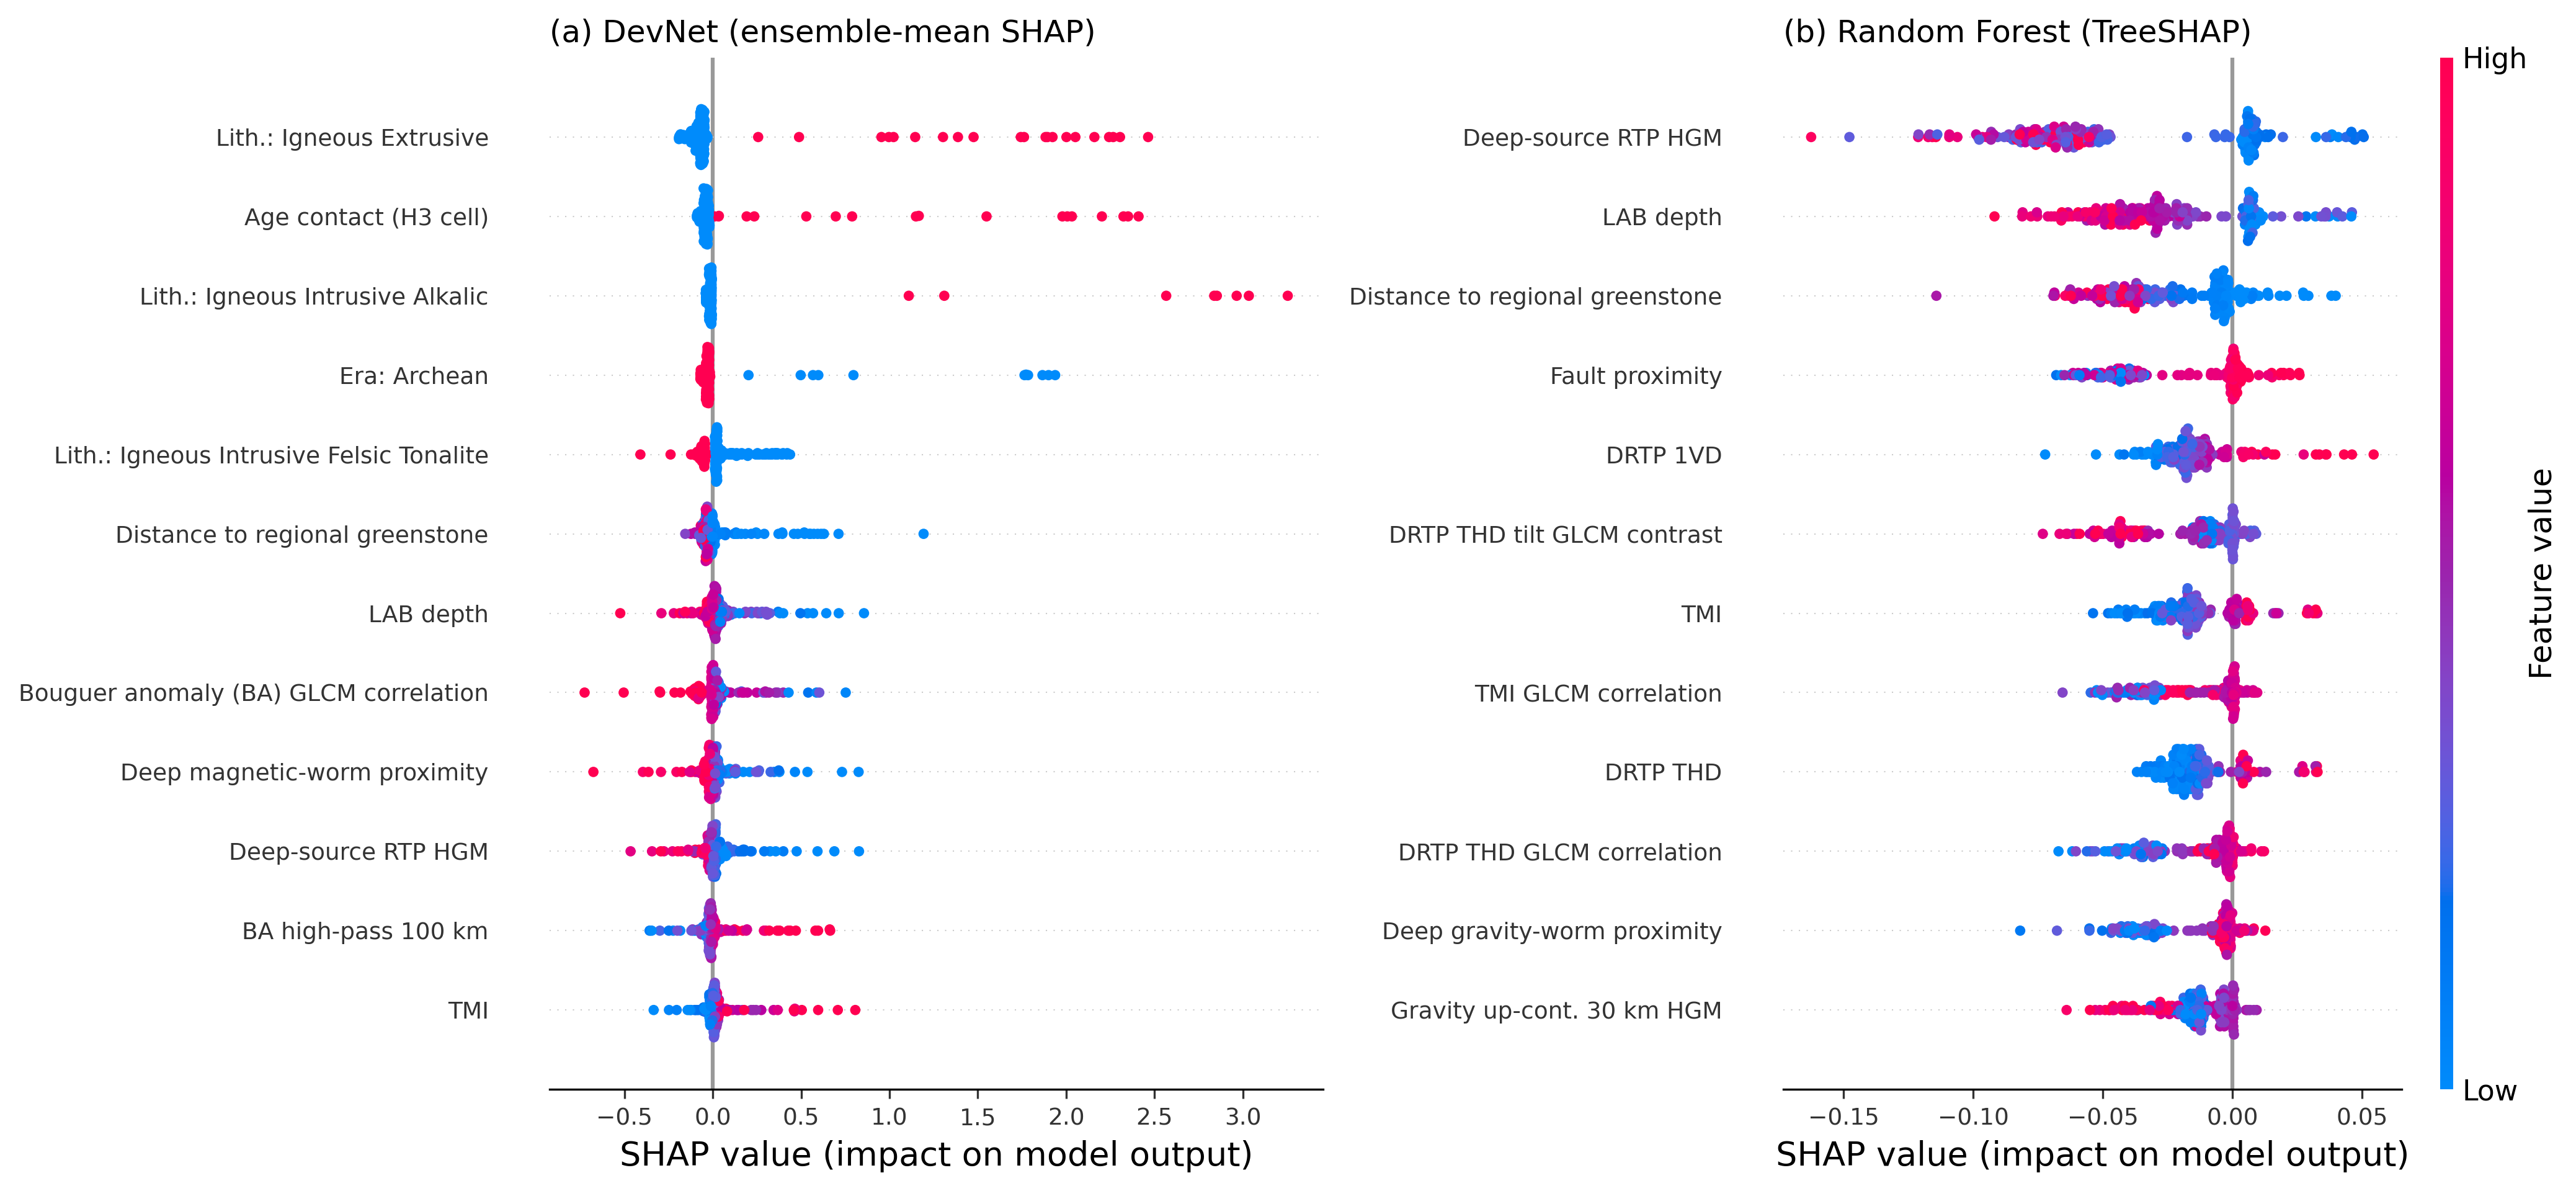
\includegraphics[width=\textwidth]{figures_r7/fig_shap_superior_r2.png}
\caption{SHAP summaries for Superior: (a) DevNet (DeepSHAP on its quantile-transformed inputs, mean over the five ensemble members) and (b) RF (TreeSHAP). Each point is one explained sample; colour is the feature value. SHAP magnitudes are not comparable between models (unbounded anomaly score vs probability).}\label{fig:shap}
\end{figure}

\begin{table}[t]
\caption{Superior: the ten jointly most important features (mean $|$SHAP$|$, normalised per model). Rank among 57 features; direction $\uparrow$/$\downarrow$: higher values (or presence) raise/lower the score, with Spearman $\rho$ between feature value and SHAP value.}\label{tab:shap}
\scriptsize
\setlength{\tabcolsep}{2.5pt}
\begin{tabular*}{\textwidth}{@{\extracolsep\fill}lcccc}
\toprule
Feature & DevNet rank & DevNet dir. & RF rank & RF dir. \\
\midrule
Deep-source RTP HGM & 10 & $\downarrow$ (-0.94) & 1 & $\downarrow$ (-0.73) \\
Lith.: Igneous Extrusive & 1 & $\uparrow$ (+0.53) & 41 & $\uparrow$ (+0.53) \\
LAB depth & 7 & $\downarrow$ (-0.93) & 2 & $\downarrow$ (-0.89) \\
Distance to regional greenstone & 6 & $\downarrow$ (-0.88) & 3 & $\downarrow$ (-0.92) \\
Age contact (H3 cell) & 2 & $\uparrow$ (+0.50) & 37 & $\uparrow$ (+0.50) \\
Lith.: Igneous Intrusive Alkalic & 3 & $\uparrow$ (+0.34) & 22 & $\uparrow$ (+0.34) \\
DRTP 1VD & 13 & $\uparrow$ (+0.95) & 5 & $\uparrow$ (+0.90) \\
TMI & 12 & $\uparrow$ (+0.93) & 7 & $\uparrow$ (+0.91) \\
Era: Archean & 4 & $\downarrow$ (-0.39) & 24 & $\downarrow$ (-0.39) \\
Fault proximity & 18 & $\uparrow$ (+0.88) & 4 & $\uparrow$ (+0.87) \\
\botrule
\end{tabular*}
\end{table}

\subsubsection{Prospectivity maps and external validation}\label{sec:res-maps}

The production DevNet and RF maps (Fig.~\ref{fig:maps}) both concentrate their highest classes in the southern Superior Province, around the eastern-Abitibi cluster and across the Abitibi and Wawa subprovinces, but their rankings of the province are only moderately similar (Spearman correlation over the grid 0.33). RF assigns a probability of exactly zero to 80\% of the grid, so its classes are drawn from the remaining nodes. In the Kapuskasing area (Fig.~\ref{fig:ksz}) DevNet places its top 1\% mainly in the Abitibi Subprovince east of the KSZ; along the KSZ itself, the top 5\% and 10\% classes form discontinuous north-north-east trending patches on its western side. Clay-Howells, the untrained Fe--REE--Nb resource on the KSZ, lies 79~km from the nearest training occurrence; among the province's 8,000 random background points the production models place it at the 96.6th (DevNet) and 99.8th (RF) percentile.

\begin{figure}[t]
\centering
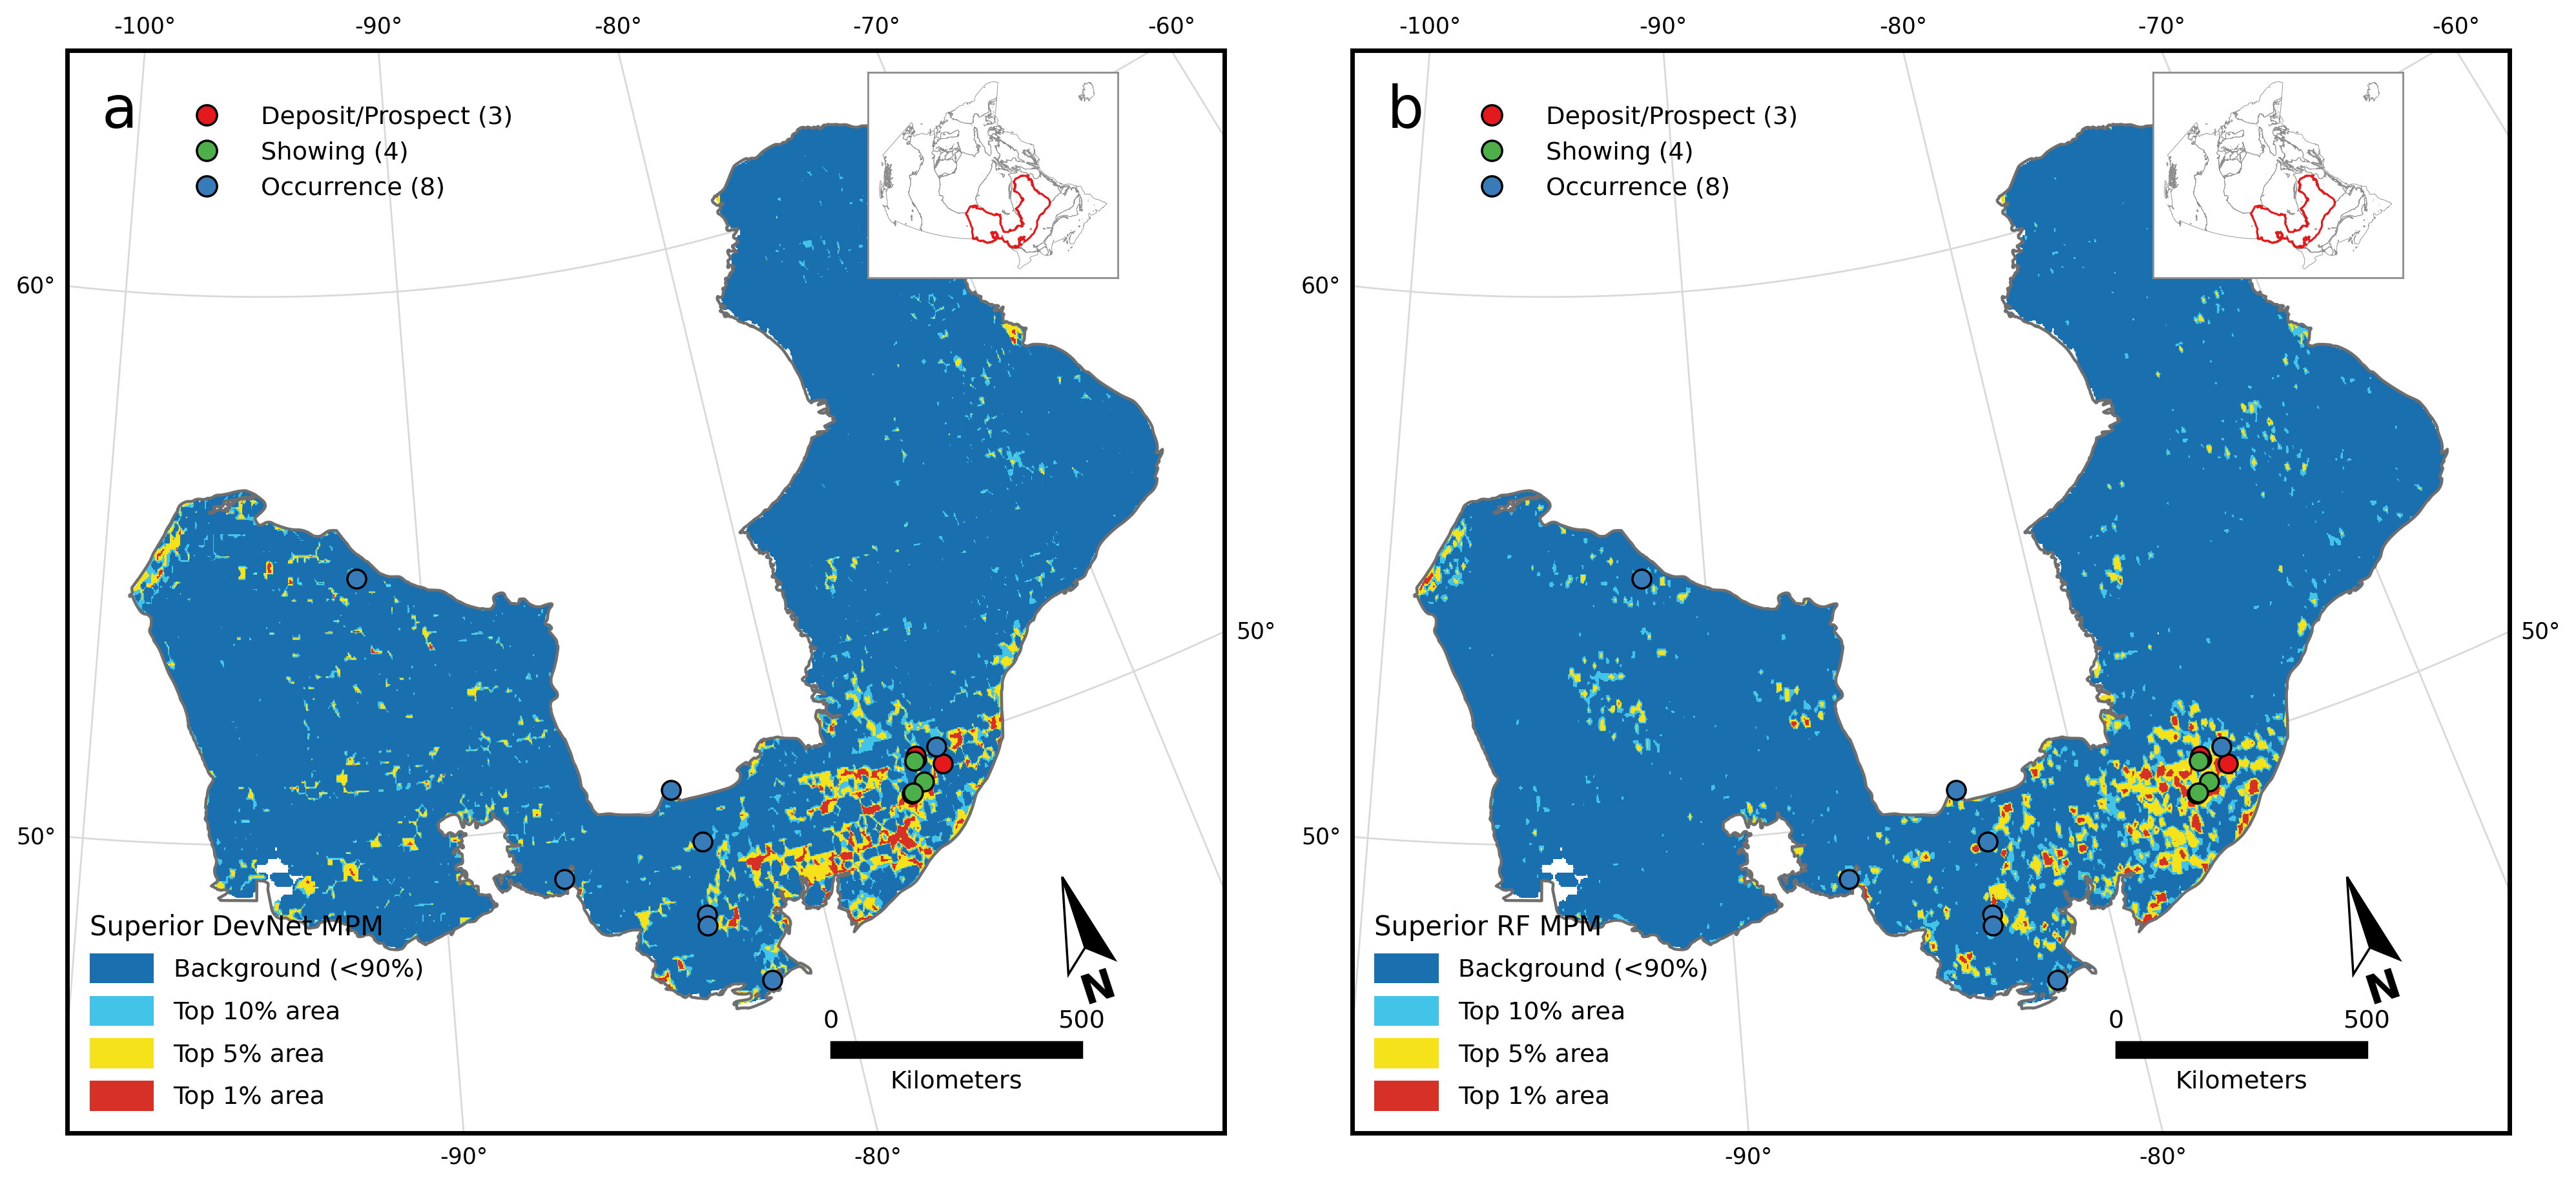
\includegraphics[width=\textwidth]{figures_r7/fig_map_superior_r2.png}
\caption{Superior prospectivity maps from the production (a) DevNet and (b) RF models, classified by score percentile over the mapped area (top 1\%, 5\% and 10\%), with known occurrences by development class (Canada Atlas Lambert). Scores on the 0.1$^\circ$ prediction grid were interpolated to a 2~km raster.}\label{fig:maps}
\end{figure}

\begin{figure}[t]
\centering
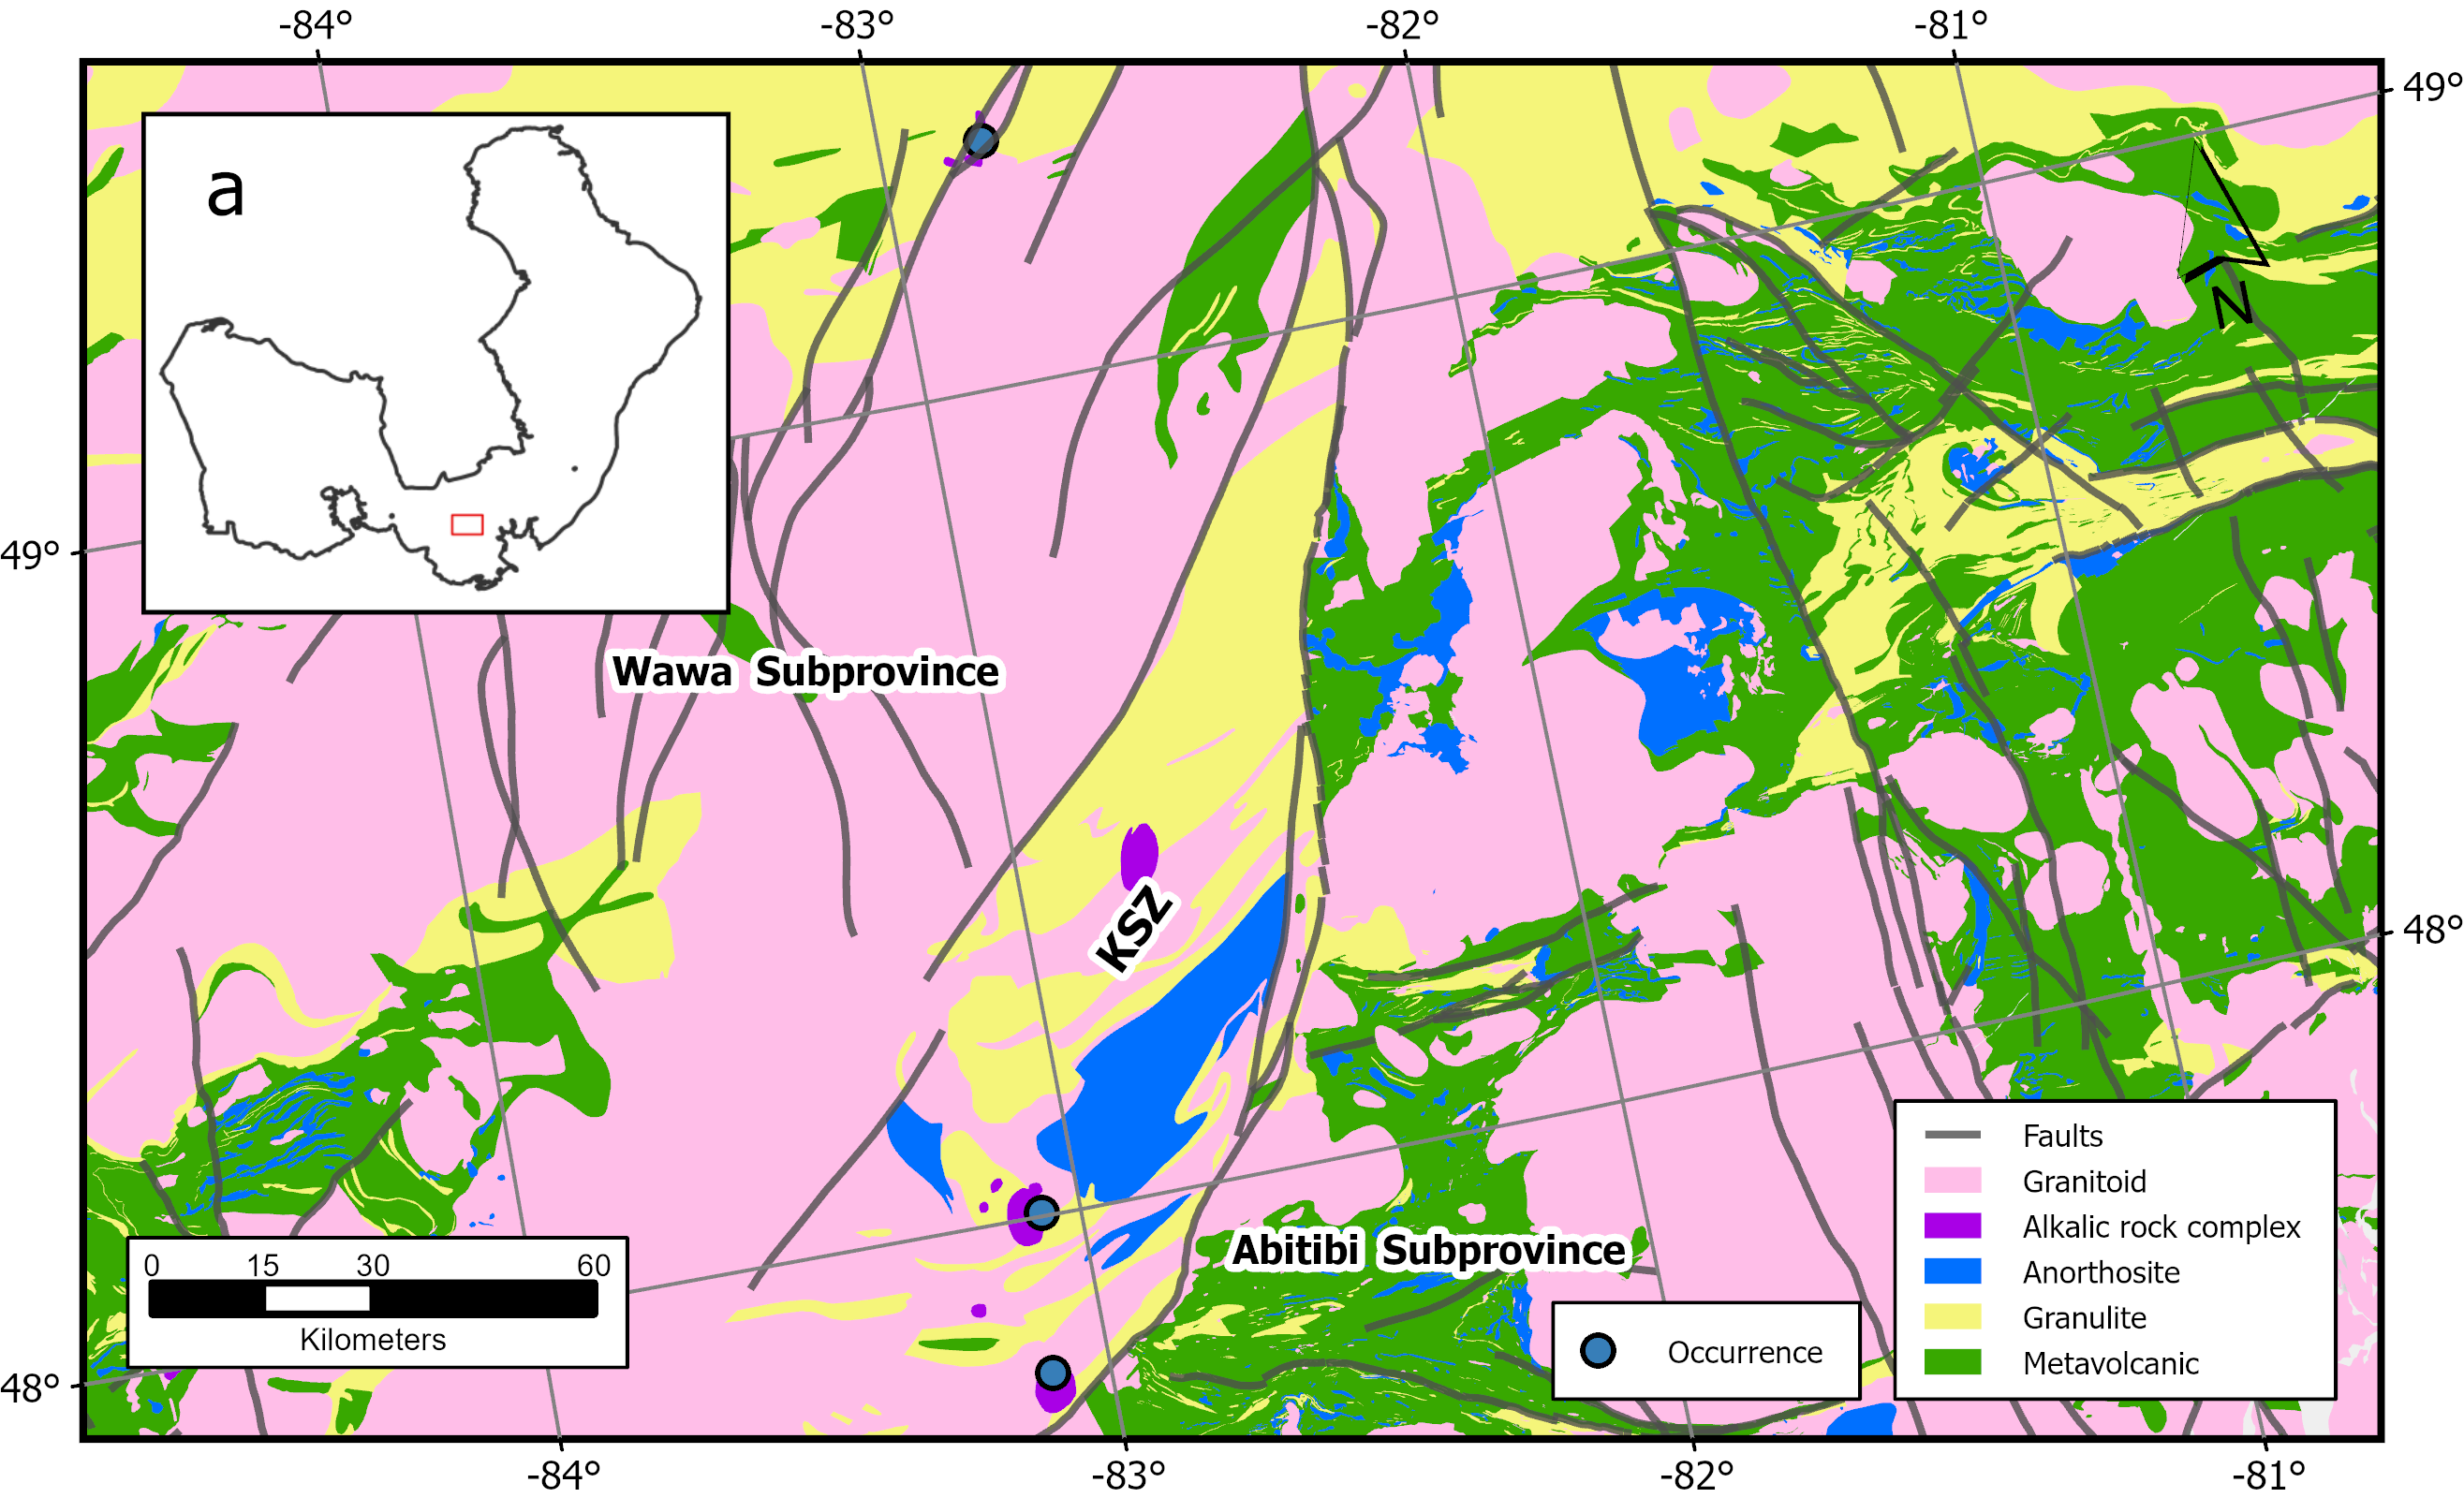
\includegraphics[width=0.49\textwidth]{figures/fig_ksz_geology.png}\hfill
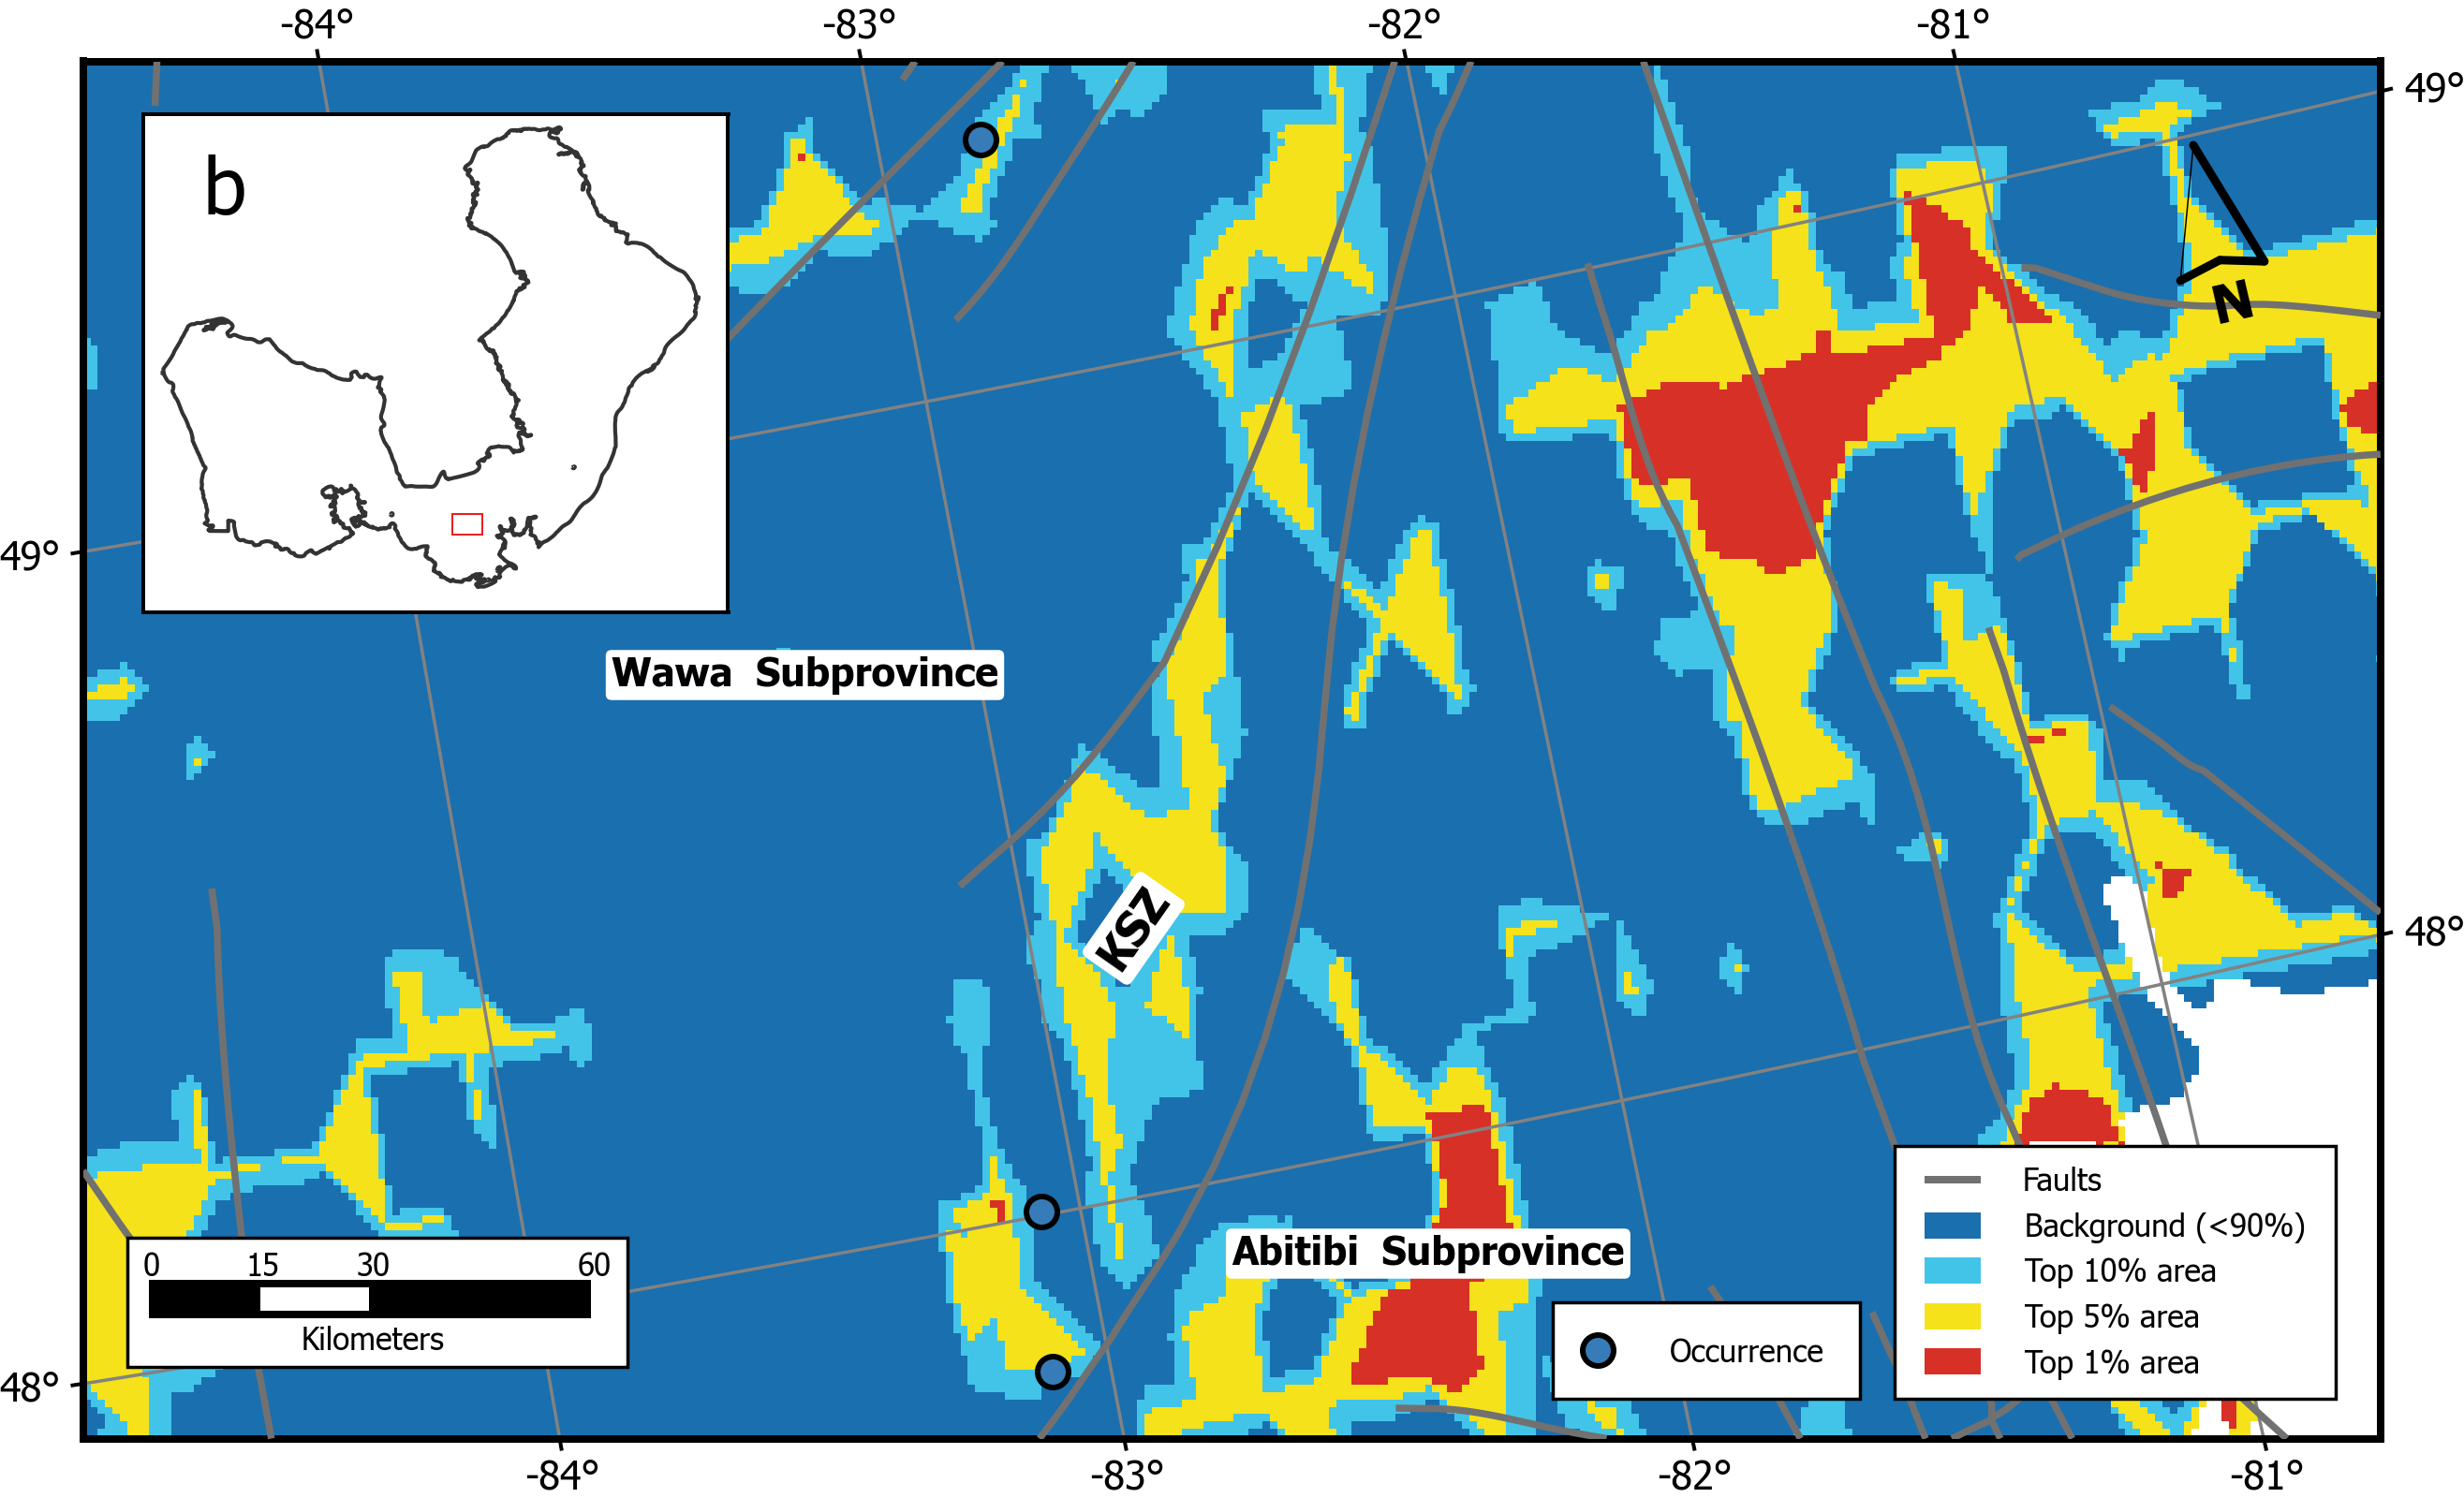
\includegraphics[width=0.49\textwidth]{figures_r7/fig_ksz_r2.png}
\caption{Kapuskasing area. (a) Regional geology with the Kapuskasing Structural Zone (KSZ) and alkalic rock complexes \citep{Gittins1967,Percival1994}, compiled from \citet{Heather1995} and \citet{Montsion2018}. (b) DevNet top 1\%, 5\% and 10\% classes (province-wide percentiles), with faults from the compilation used as an evidence layer, on the same frame as (a).}\label{fig:ksz}
\end{figure}


%% ===================================================================
\section{Discussion}\label{sec:discussion}

\subsection{National-scale models and transferability}\label{sec:disc-scale}

The national experiments explain why we model the provinces separately. First, the high test scores of the S2-grid design do not measure prediction on unexplored ground. Random splitting of augmented child cells leaves near-copies of the test positives in the training set, and negatives drawn from the least similar ground remove from evaluation exactly the ground on which a prospectivity model is hard to get right; either element alone gives a near-perfect AUC, and with one label per occurrence and random background at a realistic prevalence the same forest reaches an AP of 0.29. Second, a larger, pooled label set does not buy transferability. The provinces are separable domains, several layers mark occurrences in opposite directions (LAB and Moho depth, distance to greenstone), and models trained in one province rank another province's occurrences close to or below chance. In the terms of \citet{Meyer2021}, a province lies outside the area of applicability of a model trained on another, and pooling widens the training domain without making the model applicable to each part of it. A national model has to learn several expressions of the mineral system at once from 66 occurrences; a provincial model has to learn one.

\subsection{Performance of the deviation network}\label{sec:disc-devnet}

In Superior DevNet ranks held-out occurrences better than RF, XGBoost and bagging-PU in every repeat of every protocol, and than nnPU in all but two blocked repeats, and its lead is largest when the test requires extrapolation: RF, XGBoost and bagging-PU, which learn sharp decision boundaries around the training positives, lose 33--68\% of their AP once the nearest training occurrence is 50--200~km away, whereas DevNet keeps most of its AP to 100~km. With 15 positives the size of the margin over RF is uncertain (its 95\% intervals reach down to 0.03), and DevNet's design was chosen with these provinces in view; but the lead is consistent across all 18 repeat--block combinations.

DevNet's advantage does not hinge on its two design choices (Appendix~\ref{app:sensitivity}, Table~\ref{tab:ablation}). With z-scored inputs, label-balanced batches or ten times more steps it still ranks held-out Superior occurrences well above RF under every protocol (AP 0.369--0.417 under random splits and 0.290--0.342 with 100~km blocks, against 0.268 and 0.129 for RF), and the final configuration is the best variant only with 100 and 200~km blocks (0.345 and 0.221). What the variants share is the deviation loss and a score that is a sum of a few ReLU ridges in the space of the inputs. A smooth score of this kind is rewarded when held-out occurrences lie far from the training ones, whereas the thresholds of tree ensembles carve out the neighbourhood of each training positive.

Among the learners that treat the background as unlabelled, the deviation loss is the one that works. nnPU, which shares DevNet's network and inputs and differs only in its risk, trails it by 0.13--0.30 in AP under blocking, fails in Cordillera and Grenville and without map classes, and depends on a class prior that is unknown in practice (AP 0.145--0.275 for $\pi$ between 0.005 and 0.05); bagging-PU trails it under every protocol.

The Cordilleran and Grenville results bound the conclusion. Where positives are comparatively plentiful and clustered (Cordillera), or the geophysical signal is weak (Grenville), the tree-based learners are as good or better under random splits, and no model transfers between blocks. DevNet is therefore not a universal replacement for discriminative baselines; its advantage is specific to the combination of very few positives, a shared geological setting and the need to extrapolate within it.

\subsection{Geological map classes: evidence and lookup}\label{sec:disc-mapclasses}

The map classes move every model more than the choice of model does. Withholding them costs DevNet and RF about half or more of their AP, and a single class, alkalic intrusive rock, carries 30--49\% of DevNet's blocked AP. Six of the 15 Superior occurrences lie on cells mapped as alkalic intrusive rock, which covers 0.5\% of the background; for these occurrences the map already marks the target. The age-contact flag of the containing cell partly does the same, because a Proterozoic complex mapped within Archean crust creates an age contact, and DevNet ranks it second.

Whether such lookup is acceptable depends on the use. For targeting within mapped complexes, or for ranking known complexes by their geophysical setting, a mapped alkaline intrusion is legitimate and strong evidence, and the full inputs are appropriate. For finding complexes that the 1:5,000,000 map does not show, it is not, and the relevant skill is that without map classes: an AP of 0.075--0.123 under spatial blocking, 15--25 times the random-ranking value but well below what the full inputs suggest. Comparisons between studies, and claims about how well a model ``discovers'' occurrences, should state which of the two is being measured. In both settings DevNet is at or near the top under blocking; its absolute skill, however, depends strongly on the map classes.

\subsection{Differences between provinces}\label{sec:disc-provinces}

Grenville is the weakest of the three provinces for every model and Superior the strongest. The evidence layers are the same national compilations everywhere and almost complete (less than 0.01\% of values missing in each province), so the contrast does not reflect data coverage. It follows instead from the label sets and from the geology they sample.

First, the occurrences are less independent than their count suggests, most of all in Cordillera and Grenville: there, more than half of the occurrences lie within 10~km of another (median distance to the nearest other occurrence 7~km, against 31~km in Superior). Under a random split such neighbours fall on both sides, which is why the random-split skill in these two provinces is high and collapses under blocking (Section~\ref{sec:res-spatial}).

Second, the Grenville label set mixes carbonatites of different ages and tectonic settings. Crevier is a late-Grenvillian alkaline--carbonatite intrusion of about 957~Ma \citep{Groulier2020}. St-Honoré, with Terres Rompues on the same complex, was emplaced at about 580~Ma in the Saguenay graben of the St.~Lawrence rift system \citep{Neron2018}. The Lavergne--Springer occurrences lie near Lake Nipissing at the western end of the Ottawa--Bonnech\`ere graben, and the Cantley, Quinnville and Templeton showings near Gatineau belong to the calcite-rich veins and dykes of the Grenville marble belts, whose magmatic origin has long been debated \citep{Moecher1997}. Age diversity alone is not the problem, since the Superior occurrences also span several magmatic episodes \citep{Rukhlov2010}. They were, however, all emplaced into the same stable cratonic lithosphere, whose margins and crustal-scale structures the present-day LAB, Moho and potential-field layers still record. The Grenville crust was reworked by the Grenvillian orogeny and by later rifting, so its present-day geophysics need not record a common setting for occurrences that formed in different ones. The mapped geology adds noise of its own: the twelve Grenville occurrences fall on Archean, Proterozoic and Paleozoic map units, because the bedrock map records reworked protoliths and the Paleozoic cover over St-Honoré rather than the carbonatites, and none of them lies on a cell mapped as alkalic intrusive rock, whereas about 5\% of the Grenville background does. The same lack of a common setting, at a larger scale, is why models do not transfer between provinces (Section~\ref{sec:res-transfer}).

Missing or coarse geophysics therefore explains little of the contrast; the number, independence and geological coherence of the labels explain most of it. A model for Grenville would need either more occurrences of one carbonatite type or separate models for rift-related and orogenic types, which the present label set cannot support.

\subsection{Synthetic positives and label scarcity}\label{sec:disc-gan}

Synthetic positives are an attractive response to label scarcity, and GAN-generated labels have been recommended for exactly this commodity \citep{Parsa2025}. Our results counsel caution. A generator fitted to a dozen training positives has two options. It can stay close to them, in which case it adds near-duplicates that carry no new information (jitter and SMOTE, nearest-neighbour ratios of 0.1--0.2); or it can spread out, in which case it must guess where unseen occurrences lie and, having no information about that, places part of its mass in background-like feature space (WGAN-GP, 37\% of samples nearest to a background point). Neither option supplies the information that is actually missing, namely what undiscovered occurrences look like. The gains for RF are better explained as smoothing: synthetic points around and between the training positives make more trees vote for held-out points near them, which relieves RF's degenerate surface of exactly-zero probabilities rather than teaching it new geology. The WGAN-GP samples, which spread furthest, help RF most, also with 200~km blocks, yet even the best augmented RF stays well below DevNet without augmentation (0.191 against 0.345 with 100~km blocks), and DevNet, whose loss already produces smooth scores, gains little and inconsistently from the same points. Where synthetic positives are used, they must be generated inside each training fold from that fold's positives only, and performance must be measured on real held-out occurrences; otherwise a synthetic copy of a training occurrence in the test set reproduces the sibling problem of Section~\ref{sec:res-ladder} in another form.

\subsection{Validation design and reported performance}\label{sec:disc-protocol}

Four of our findings concern evaluation rather than models. First, with tens of positives a single cross-validation split gives a noisy estimate: re-splitting the same Superior data moves each model's AP over a range of 0.06--0.11 (Table~\ref{tab:benchmark}), as large as many of the differences between models. Second, random splits overstate skill wherever occurrences cluster, and the size of the overstatement differs between models, so random splits can also reverse a model ranking (Section~\ref{sec:res-spatial}). Third, rebuilt nationally, the S2-grid design gives a test AUC of 1.000, and two of its elements each suffice for it: splitting augmented child cells at random (0.997 with random negatives), because almost every test positive has a sibling, sharing the coarse deep-architecture values and the map classes exactly and the fine-scale values nearly, on the training side; and drawing negatives from the least similar ground (0.998 without augmentation). In this design the held-out test asks the model to recognise a location it has already seen, and the comparison of training and test AUC, which \citet{Parsa2024} used to argue that their models were not over-fitted, becomes uninformative because the test set is not independent of the training set. Selecting negatives from the least similar 5\% of the ground adds a second, independent source of optimism: it removes from evaluation exactly the ground on which a prospectivity model is hardest to get right. Fourth, the geological map classes can supply a large share of the reported skill by marking known complexes (Section~\ref{sec:disc-mapclasses}), which no split design removes.

We stress what the national experiment does and does not show. It uses our inputs and labels, and the random forest of \citet{Parsa2024} rather than their best model, a CNN, and it does not establish what their numbers would have been under a grouped split. It does show that, on national Canadian carbonatite data, the published design produces a test AUC of 1.000, whereas the same forest with one label per occurrence, random background and a realistic prevalence reaches an AUC of 0.903 and an AP of 0.292, and that a model trained in one province does not carry over to another. Neither the high AUC nor its small spread over splits can be taken as evidence of generalisation to unexplored ground. \citet{Parsa2025} describe the same stratified random 70/30 split for a workflow that adds GAN-generated labels; their description does not state whether synthetic labels derived from an original label were kept on the same side of the split as that label. If they were not, the caveat applies with greater force. For prospectivity studies under extreme label scarcity we therefore recommend (i) grouping every augmented or near-duplicate label with its source occurrence before any split, (ii) drawing evaluation negatives at random from the domain rather than from the ground least similar to the positives, (iii) reporting AP with intervals over repeated splits rather than a single AUC, (iv) adding a spatially blocked validation in which training background is purged from held-out blocks, (v) reporting results with and without point-level map classes, so that readers can see how much of a score is map lookup, and (vi) for models pooled across geological provinces, testing transfer to held-out provinces and computing extent-dependent inputs within fixed geological units.

\subsection{Geological interpretation}\label{sec:disc-geology}

The drivers on which RF and DevNet agree in Superior describe a coherent setting. Shallower LAB, together with the strong ranking of deep-source magnetic gradients, points to the thinner lithosphere at the edges of the thick Superior root, where small-degree melting of metasomatised mantle and access along lithosphere-scale structures are most likely \citep{Griffin2013,Groves2021,Hoggard2020}; a mantle conductor beneath the southern Abitibi is consistent with such metasomatism \citep{Snyder2021}. Fault proximity and high magnetic intensity capture the structures that focus ascent and the magnetite-bearing intrusions themselves \citep{Thomas2016}. The negative effect of proximity to deep magnetic worms is less intuitive; it may reflect the concentration of deep magnetic contacts along terrane boundaries that are not themselves carbonatite hosts, and should not be over-interpreted.

The strong positive effect of greenstone lithology and of proximity to regional greenstone units needs more care. Eight of the 15 occurrences belong to the eastern-Abitibi cluster in a greenstone-dominated subprovince, so the association may partly record where the largest cluster lies rather than a control shared by the dispersed occurrences; the dispersed occurrences that DevNet ranks lowest under blocking, Kapuskasing and Nemegosenda Lake, lie in the high-grade and alkaline terrain of the KSZ rather than in a greenstone belt. Consistent with this, DevNet's map follows the KSZ only in discontinuous patches, while the untrained Clay-Howells resource on the KSZ still ranks at its 97th percentile. A model whose top classes are tied to one greenstone-hosted cluster is useful for ranking ground of that type, but it should not be expected to recognise alkaline complexes in other settings as well.

\subsection{Limitations}\label{sec:limitations}

Fifteen positives allow only weak statistical statements: our firm results are those that are consistent across repeats, block sizes, comparisons and provinces. DevNet's input representation and batch composition were chosen with diagnostic experiments on these three provinces, although with the present inputs every variant ranks Superior occurrences above RF (Appendix~\ref{app:sensitivity}); confirmation on an independent province is needed, and the Churchill Province, the obvious candidate, holds too few carbonatite-hosted occurrences after deduplication for a meaningful test. The geological encoding used here replaced a coarser grouping of lithologies after that grouping had been evaluated; the change raised the AP of every model except nnPU under random splits and 50--100~km blocks but not with 200~km blocks. The evaluation background may contain undiscovered occurrences, so all metrics are lower bounds. Radiometric data could not be used because of incomplete coverage, and whole-rock geochemistry is too sparse to serve as an input. The reduction to the pole assumes induced magnetisation; remanently magnetised bodies are not reduced correctly. The provenance of the fault compilation should be confirmed against the original data release before publication. The occurrence-class information (Deposit/Prospect, Showing, Occurrence) was not used for weighting; with 3--8 occurrences per class, confidence-weighted training could not be evaluated reliably. Finally, maps are per-region percentiles and are not calibrated probabilities. At the national scale, 12 of the 66 occurrences lie outside the three study provinces and four of them form one cluster (Ashram), so the ``rest of Canada'' group is small and spatially dependent; the national labels come from two compilations: a third \citep{Huston2024}, used by a parallel national study, would add one deposit (Hoidas Lake), and the five records of \citet{Orris2018} whose carbonatite affinity is marked as uncertain, which we excluded, would add five more (one of them Clay-Howells, our external check); and the 0.1$^\circ$ lattice samples high latitudes more densely per unit area.

%% ===================================================================
\section{Conclusions}\label{sec:conclusions}

For carbonatite-hosted REE prospectivity mapping in Canada, with 66 occurrences nationally and 12--27 per province:
\begin{enumerate}
\item Rebuilt on these data, the national S2-grid design of \citet{Parsa2024} gives a test AUC of 1.000; random splitting of augmented child cells and negatives drawn from the least similar ground each suffice for it. With one label per occurrence, random background and a realistic prevalence, the same forest reaches an AUC of 0.903 and an AP of 0.292.
\item Models do not transfer between geological provinces: a province's model ranks another province's occurrences at or below chance in most cases, the provinces are separable in the evidence layers, and several layers mark occurrences in opposite directions in different provinces. Prospectivity models for these occurrences should therefore be built per province.
\item In the Superior Province a semi-supervised Deviation Network ranks held-out occurrences better than Random Forest, XGBoost, bagging-PU and nnPU under random and 50--200~km spatially blocked cross-validation (AP 0.38 and 0.37--0.22 against 0.27 and 0.18--0.09 for RF and XGBoost), in every repeat against RF, XGBoost and bagging-PU; with 15 occurrences the margin over RF is consistent but its size is uncertain. The advantage does not depend on DevNet's input scaling or batch composition.
\item Geological map classes move every model more than the choice of model. A single mapped alkalic-intrusion class, covering 6 of 15 Superior occurrences and 0.5\% of the background, carries 30--49\% of DevNet's blocked AP, and without point-level map classes DevNet and RF lose about half or more of their skill. Prospectivity studies should report results with and without such classes.
\item In the Cordilleran Orogen and the Grenville Province the tree-based learners lead under random splits and no model transfers between blocks; the number, independence and geological coherence of the labels, not data coverage, explain the contrast.
\item Synthetic positives from jitter, SMOTE or a tabular WGAN-GP, generated strictly within training folds, gave DevNet no consistent gain and raised RF's AP, most with WGAN-GP, without bringing it close to unaugmented DevNet.
\item RF and DevNet agree on the direction of all 30 leading drivers across the three provinces. DevNet's Superior map places the untrained Clay-Howells Fe--REE--Nb resource at its 97th percentile and favours greenstone-hosted settings like the dominant Abitibi cluster.
\end{enumerate}

\backmatter

\bmhead{Acknowledgements}
This work began as an MSc Independent Research Project at Imperial College London. We thank Ross Smail, Prof. Chetan Nathwani and Prof. Rebecca Bell for supervision, and Junlin Fang for discussions on methodology and model evaluation.

\section*{Declarations}

\bmhead{Funding} %% TODO(author)
Not applicable.

\bmhead{Competing interests} %% TODO(author)
The authors declare no competing interests.

\bmhead{Data availability}
Occurrence labels are derived from \citet{Orris2018} and \citet{Parsa2024}; the deduplicated provincial and national tables and the study-area outlines are distributed with the code. All evidence layers are public and available from \citet{McCafferty2023}, \citet{Jobin2017}, \citet{Miles2016}, \citet{BradleyDC2008} and \citet{Wheeler1996}; the derived gravity and magnetic grids are reproduced by the code.

\bmhead{Code availability} %% TODO(author): make the repository public or archive it (e.g. Zenodo) before submission
The pipeline, every analysis in this paper and the scripts that generate its tables and figures are available at \url{https://github.com/miaozhou-312/ree-prospectivity-paper}.

\begin{appendices}

\section{Additional results}\label{app:full}

\begin{table}[!h]
\caption{AUC (median over six repeats) for the runs of Table~\ref{tab:spatial}. Bold: highest AUC in each row.}\label{tab:spatial-auc}
\footnotesize
\setlength{\tabcolsep}{3pt}
\begin{tabular*}{\textwidth}{@{\extracolsep\fill}llccccc}
\toprule
Region & Split & DevNet & RF & XGBoost & Bagging-PU & nnPU \\
\midrule
\multirow{4}{*}{Superior} & random & 0.972 & \textbf{0.985} & 0.976 & 0.976 & 0.842 \\
 & 50 km & 0.969 & \textbf{0.976} & 0.962 & 0.964 & 0.862 \\
 & 100 km & \textbf{0.928} & 0.922 & 0.904 & 0.921 & 0.846 \\
 & 200 km & \textbf{0.886} & 0.861 & 0.826 & 0.837 & 0.819 \\
\midrule
\multirow{4}{*}{Cordillera} & random & 0.925 & 0.936 & 0.926 & \textbf{0.937} & 0.575 \\
 & 50 km & 0.866 & 0.856 & 0.840 & \textbf{0.879} & 0.581 \\
 & 100 km & 0.747 & 0.841 & 0.782 & \textbf{0.856} & 0.565 \\
 & 200 km & 0.744 & 0.720 & 0.712 & \textbf{0.825} & 0.584 \\
\midrule
\multirow{4}{*}{Grenville} & random & 0.826 & 0.836 & 0.870 & \textbf{0.909} & 0.609 \\
 & 50 km & 0.755 & 0.717 & 0.777 & \textbf{0.825} & 0.620 \\
 & 100 km & 0.699 & 0.687 & 0.722 & \textbf{0.780} & 0.598 \\
 & 200 km & 0.681 & 0.582 & 0.665 & \textbf{0.691} & 0.609 \\
\botrule
\end{tabular*}
\end{table}

\begin{table}[!h]
\caption{Sensitivity of nnPU to the assumed class prior $\pi$, Superior (random cross-validation; median and 95\% interval over six repeats).}\label{tab:prior}
\footnotesize
\begin{tabular*}{0.6\textwidth}{@{\extracolsep\fill}lcc}
\toprule
$\pi$ & AUC & AP \\
\midrule
0.005 & 0.823 [0.761, 0.860] & 0.145 [0.079, 0.177] \\
0.01 & 0.842 [0.772, 0.873] & 0.159 [0.096, 0.210] \\
0.02 & 0.864 [0.827, 0.897] & 0.195 [0.115, 0.251] \\
0.05 & 0.885 [0.878, 0.919] & 0.275 [0.186, 0.395] \\
\botrule
\end{tabular*}
\end{table}

\clearpage
\section{Synthetic positives: generators and spatial blocking}\label{app:aug-spatial}

\begin{figure}[!h]
\centering
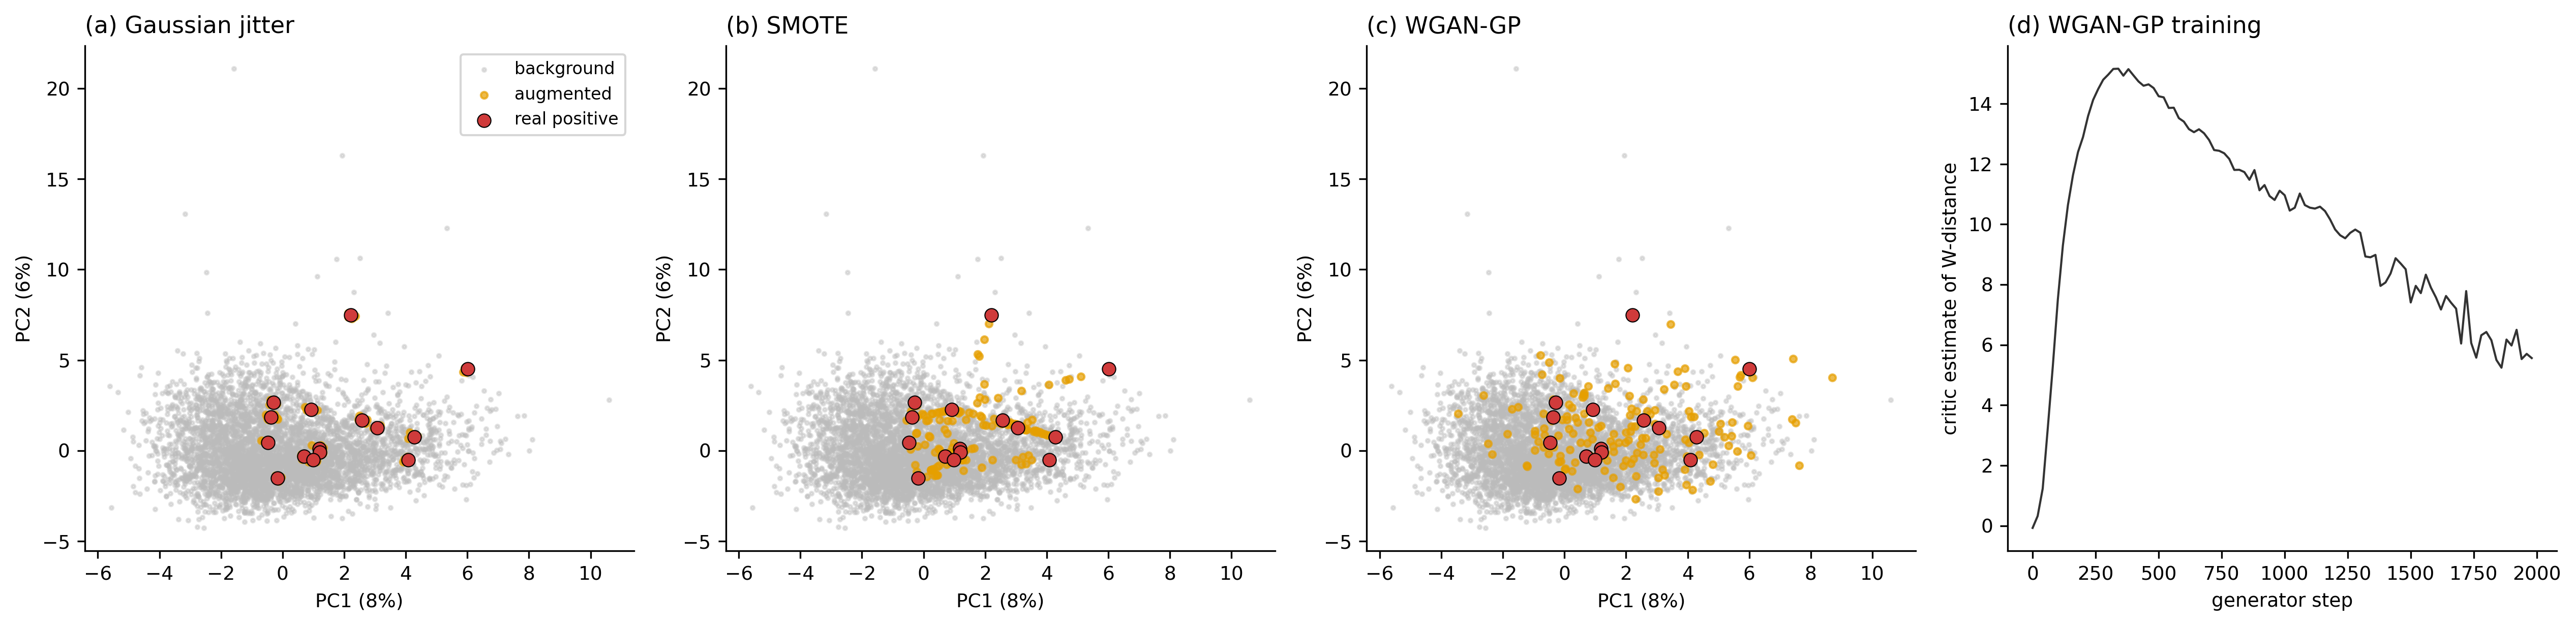
\includegraphics[width=\textwidth]{figures_r7/fig_augmentation_superior_r4.png}
\caption{(a--c) Synthetic positives from each generator (fitted to all 15 Superior positives) in the first two principal components of background and real positives. (d) WGAN-GP critic estimate of the Wasserstein distance during training.}\label{fig:aug-pca}
\end{figure}


\begin{table}[!h]
\caption{Superior average precision with fold-safe synthetic positives under spatially blocked cross-validation (median and 95\% interval over six repeats). DevNet's runs were computed on a second machine; its training is not bit-for-bit identical across machines, so its unaugmented values differ from Table~\ref{tab:spatial} in the third decimal.}\label{tab:aug-spatial}
\footnotesize
\begin{tabular*}{0.7\textwidth}{@{\extracolsep\fill}lllc}
\toprule
Blocks & Model & Augmentation & AP \\
\midrule
100 km & DevNet & none & 0.343 [0.163, 0.414] \\
 &  & Gaussian jitter 10$\times$ & 0.341 [0.156, 0.420] \\
 &  & SMOTE 3$\times$ & 0.324 [0.146, 0.418] \\
 &  & WGAN-GP 3$\times$ & 0.326 [0.228, 0.398] \\
 &  & WGAN-GP 10$\times$ & 0.308 [0.172, 0.350] \\
\addlinespace
100 km & RF & none & 0.129 [0.067, 0.161] \\
 &  & Gaussian jitter 10$\times$ & 0.139 [0.074, 0.187] \\
 &  & SMOTE 3$\times$ & 0.110 [0.053, 0.168] \\
 &  & WGAN-GP 3$\times$ & 0.135 [0.074, 0.202] \\
 &  & WGAN-GP 10$\times$ & 0.191 [0.083, 0.294] \\
\addlinespace
200 km & DevNet & none & 0.216 [0.154, 0.310] \\
 &  & Gaussian jitter 10$\times$ & 0.238 [0.157, 0.314] \\
 &  & SMOTE 3$\times$ & 0.200 [0.155, 0.251] \\
 &  & WGAN-GP 3$\times$ & 0.246 [0.165, 0.314] \\
 &  & WGAN-GP 10$\times$ & 0.258 [0.171, 0.305] \\
\addlinespace
200 km & RF & none & 0.087 [0.053, 0.149] \\
 &  & Gaussian jitter 10$\times$ & 0.096 [0.062, 0.137] \\
 &  & SMOTE 3$\times$ & 0.077 [0.047, 0.118] \\
 &  & WGAN-GP 3$\times$ & 0.132 [0.080, 0.199] \\
 &  & WGAN-GP 10$\times$ & 0.122 [0.074, 0.256] \\
\botrule
\end{tabular*}
\end{table}

\clearpage
\section{Interpretation in the contrasting provinces}\label{app:shap}

\begin{table}[!h]
\caption{As Table~\ref{tab:shap}, Cordillera (61 features).}\label{tab:shap-cord}
\footnotesize
\begin{tabular*}{\textwidth}{@{\extracolsep\fill}lcccc}
\toprule
Feature & DevNet rank & DevNet dir. & RF rank & RF dir. \\
\midrule
Distance to regional high-grade metam. & 5 & $\downarrow$ (-0.96) & 1 & $\downarrow$ (-0.86) \\
Era: Proterozoic & 2 & $\uparrow$ (+0.59) & 19 & $\uparrow$ (+0.70) \\
Era: Mesozoic & 4 & $\downarrow$ (-0.82) & 11 & $\downarrow$ (-0.82) \\
Bouguer anomaly (BA) & 9 & $\downarrow$ (-0.96) & 3 & $\downarrow$ (-0.87) \\
Age contact (H3 cell) & 1 & $\uparrow$ (+0.84) & 44 & $\uparrow$ (+0.84) \\
DRTP THD GLCM correlation & 3 & $\downarrow$ (-0.82) & 27 & $\downarrow$ (-0.42) \\
Moho depth & 8 & $\uparrow$ (+0.96) & 6 & $\uparrow$ (+0.91) \\
Distance to regional greenstone & 17 & $\uparrow$ (+0.93) & 4 & $\uparrow$ (+0.34) \\
Passive-margin proximity & 41 & $\uparrow$ (+0.28) & 2 & $\uparrow$ (+0.81) \\
Distance to regional age contact & 7 & $\uparrow$ (+0.95) & 14 & $\uparrow$ (+0.92) \\
\botrule
\end{tabular*}
\end{table}

\begin{table}[!h]
\caption{As Table~\ref{tab:shap}, Grenville (66 features).}\label{tab:shap-gren}
\footnotesize
\begin{tabular*}{\textwidth}{@{\extracolsep\fill}lcccc}
\toprule
Feature & DevNet rank & DevNet dir. & RF rank & RF dir. \\
\midrule
Distance to regional age contact & 9 & $\downarrow$ (-0.96) & 1 & $\downarrow$ (-0.79) \\
Deep-source RTP & 5 & $\uparrow$ (+0.93) & 2 & $\uparrow$ (+0.73) \\
DRTP THD tilt & 10 & $\downarrow$ (-0.95) & 3 & $\downarrow$ (-0.83) \\
DRTP THD tilt GLCM contrast & 1 & $\downarrow$ (-0.94) & 10 & $\downarrow$ (-0.93) \\
BA THD tilt GLCM contrast & 4 & $\uparrow$ (+0.97) & 5 & $\uparrow$ (+0.83) \\
Distance to regional mafic-ultramafic & 24 & $\uparrow$ (+0.92) & 4 & $\uparrow$ (+0.42) \\
Distance to regional sedimentary & 15 & $\downarrow$ (-0.95) & 6 & $\downarrow$ (-0.90) \\
DRTP mean (10 km) & 6 & $\uparrow$ (+0.95) & 9 & $\uparrow$ (+0.93) \\
Moho depth & 22 & $\downarrow$ (-0.92) & 7 & $\downarrow$ (-0.69) \\
Deep magnetic-worm proximity & 3 & $\uparrow$ (+0.97) & 25 & $\uparrow$ (+0.79) \\
\botrule
\end{tabular*}
\end{table}

\clearpage
\section{Ablation of DevNet design choices}\label{app:sensitivity}

DevNet's two design choices (Section~\ref{sec:models}) are examined here with the inputs of the main analysis, by changing one element at a time from a configuration with z-scored inputs and label-balanced batches of 16 + 16 rows. All configurations are evaluated with the folds, protocols and seeds of the main results (Table~\ref{tab:ablation}). In Superior the variants differ little, and none is best under every protocol: under random splits z-scored inputs with background-heavy batches give the highest AP (0.417 against 0.381 for the final configuration), under 50~km blocks label-balanced batches do (0.390 and 0.384 against 0.371), and with 100 and 200~km blocks the final configuration is highest (0.345 and 0.221). Every variant stays well above RF (0.268, 0.165, 0.129 and 0.087; Table~\ref{tab:spatial}). Training for longer repeats the dozen positives and pushes the network towards memorising their neighbourhoods: with z-scored inputs, ten times more steps raised random-split AP (0.401 against 0.369) but lowered it under 100~km blocks (0.290 against 0.329). The nested early-stopping configuration chooses the number of steps (100--3,000, cosine schedule over 3,000 steps) inside each outer training fold by a 100~km spatial cross-validation (three inner folds, two inner restarts, background purged from inner validation blocks), so the test fold is never used for the choice. Table~\ref{tab:margin} gives the sensitivity of the final configuration to the deviation margin: smaller margins gave higher AP in Superior and Cordillera (Superior 0.472 with $a = 2$ against 0.381 with $a = 5$) but not in Grenville, and we keep the value of \citet{Pang2019} rather than tune it on these folds.

\begin{table}[!h]
\caption{Ablation of DevNet's design choices: AP (median over six repeats) under random cross-validation and spatial blocks, on identical folds. Inputs: quantile-normal or z-scored; batch: positive\,+\,background rows per step; steps: number of gradient steps (nested ES: chosen by nested 100~km spatial cross-validation). Bold: the final configuration. --: not run.}\label{tab:ablation}
\scriptsize
\setlength{\tabcolsep}{2.5pt}
\begin{tabular*}{\textwidth}{@{\extracolsep\fill}llllllll}
\toprule
Region & Inputs & Batch & Steps & random & 50 km & 100 km & 200 km \\
\midrule
\multirow{6}{*}{Superior} & quantile & 16\,+\,240 & 300 (final) & \textbf{0.381} & \textbf{0.371} & \textbf{0.345} & \textbf{0.221} \\
 & z-score & 16\,+\,240 & 300 & 0.417 & 0.378 & 0.342 & 0.212 \\
 & quantile & 16\,+\,16 & 300 & 0.397 & 0.384 & 0.329 & 0.220 \\
 & z-score & 16\,+\,16 & 300 & 0.369 & 0.390 & 0.329 & 0.201 \\
 & z-score & 16\,+\,16 & 3,000 & 0.401 & -- & 0.290 & -- \\
 & z-score & 16\,+\,16 & nested ES & 0.401 & 0.358 & 0.297 & 0.190 \\
\midrule
\multirow{6}{*}{Cordillera} & quantile & 16\,+\,240 & 300 (final) & \textbf{0.327} & \textbf{0.131} & \textbf{0.048} & \textbf{0.056} \\
 & z-score & 16\,+\,240 & 300 & 0.303 & 0.136 & 0.074 & 0.049 \\
 & quantile & 16\,+\,16 & 300 & 0.307 & 0.124 & 0.045 & 0.052 \\
 & z-score & 16\,+\,16 & 300 & 0.273 & 0.135 & 0.077 & 0.045 \\
 & z-score & 16\,+\,16 & 3,000 & 0.255 & -- & 0.060 & -- \\
 & z-score & 16\,+\,16 & nested ES & 0.284 & 0.140 & 0.069 & 0.047 \\
\midrule
\multirow{6}{*}{Grenville} & quantile & 16\,+\,240 & 300 (final) & \textbf{0.127} & \textbf{0.036} & \textbf{0.008} & \textbf{0.007} \\
 & z-score & 16\,+\,240 & 300 & 0.113 & 0.030 & 0.007 & 0.006 \\
 & quantile & 16\,+\,16 & 300 & 0.113 & 0.031 & 0.008 & 0.008 \\
 & z-score & 16\,+\,16 & 300 & 0.078 & 0.026 & 0.009 & 0.008 \\
 & z-score & 16\,+\,16 & 3,000 & 0.129 & -- & 0.010 & -- \\
 & z-score & 16\,+\,16 & nested ES & 0.107 & 0.022 & 0.008 & 0.008 \\
\botrule
\end{tabular*}
\end{table}

\begin{table}[!h]
\caption{Sensitivity of DevNet to the deviation margin $a$ (AP, median over six repeats, random cross-validation). The main results use $a = 5$.}\label{tab:margin}
\footnotesize
\begin{tabular*}{0.7\textwidth}{@{\extracolsep\fill}lcccc}
\toprule
Region & $a = 2$ & $a = 3$ & $a = 5$ & $a = 8$ \\
\midrule
Superior & 0.472 & 0.446 & 0.381 & 0.377 \\
Cordillera & 0.367 & 0.379 & 0.327 & 0.313 \\
Grenville & 0.126 & 0.115 & 0.127 & 0.120 \\
\botrule
\end{tabular*}
\end{table}

\end{appendices}

\clearpage

\bibliography{references}

\end{document}
